\documentclass[11pt,a4paper]{article}
\usepackage[margin=1.9cm, top=2.1cm, bottom=2.0cm]{geometry}
\usepackage[T1]{fontenc}
\usepackage{lmodern}
\usepackage{amsmath,amssymb}
\usepackage{enumitem,booktabs,array,tabularx,multirow}
\usepackage[normalem]{ulem}
\usepackage{adjustbox}
\usepackage{xcolor}
\usepackage{fancyhdr,lastpage}
\usepackage[most]{tcolorbox}
\usepackage{tikz}
\usetikzlibrary{shapes.geometric,arrows.meta,positioning,calc}
\usepackage[hidelinks]{hyperref}
\setlength{\parindent}{0pt}
\setlength{\parskip}{4pt}
\renewcommand{\arraystretch}{1.25}
\emergencystretch=2em
\pagestyle{fancy}\fancyhf{}
\lhead{\small\textit{Course: CS420 -- Artificial Intelligence}}
\rhead{\small Practice Test 4 -- Solution}
\cfoot{\small Page \thepage\ of \pageref{LastPage}}
\renewcommand{\headrulewidth}{0.4pt}
% empty answer box (exam) / filled box (solution)
\newtcolorbox{ansbox}[1][]{enhanced, breakable, colback=white, colframe=black!55, boxrule=0.5pt, arc=0pt,
  left=5pt, right=5pt, top=3pt, bottom=3pt, before skip=3pt, after skip=6pt, #1}
\newtcolorbox{solbox}{enhanced, breakable, colback=blue!2!white, colframe=blue!50!black, boxrule=0.6pt, arc=0pt,
  left=6pt, right=6pt, top=4pt, bottom=4pt, before skip=3pt, after skip=8pt,
  fontupper=\color{black}}
\newcommand{\question}[1]{\par\medskip\noindent\textbf{Question #1.}\ }
\newcommand{\subq}[1]{\par\smallskip\noindent\textbf{#1}\ }
\newcommand{\T}{\textbf{\textcolor{green!45!black}{TRUE}}}
\newcommand{\F}{\textbf{\textcolor{red!70!black}{FALSE}}}

\tikzset{
  maxn/.style={draw, thick, regular polygon, regular polygon sides=3, minimum size=10.5mm, inner sep=0pt, font=\small},
  minn/.style={maxn, shape border rotate=180},
  chn/.style={draw, thick, circle, minimum size=9.5mm, inner sep=0pt, font=\small},
  leafn/.style={draw, rectangle, minimum width=5.5mm, minimum height=5.5mm, inner sep=1pt, font=\small},
  gone/.style={draw=black!25, text=black!35},
  cut/.style={red!80!black, very thick, dashed},
  sol/.style={text=blue!70!black, font=\small\bfseries},
}

\begin{document}


{\large\textbf{\textit{Course: CS420 -- Artificial Intelligence}}}\par
{\textbf{\textit{Midterm examination review -- Lectures 0 to 3}}}\par
\begin{center}{\Large\bfseries PRACTICE MIDTERM EXAMINATION -- TEST 4\\[2pt]\textcolor{blue!55!black}{SOLUTION}}\\[3pt]
{\small Duration: 120 minutes \quad$\cdot$\quad Closed book \quad$\cdot$\quad Calculator allowed}\end{center}
\noindent\rule{\linewidth}{0.6pt}

{\small\textit{Unless a question says otherwise, ties are broken in alphabetical order (left-to-right in trees), and successors are generated in alphabetical order.}}\par
\question{1}\textit{Vacuum world with three cells.} A vacuum-cleaner robot lives in a row of \textbf{three} cells (1, 2, 3). Each cell is either dirty or clean. The robot can move Left, move Right, or Suck (clean its current cell).
\subq{(a)}Consider a state as a tuple of values. Which values should be included in the tuple?
\begin{solbox}
$(\ell, d_1, d_2, d_3)$: robot location $\ell\in\{1,2,3\}$ and the dirt status of each cell.
\end{solbox}
\subq{(b)}Define the initial state (robot in cell 1, all cells dirty) and the goal state(s).
\begin{solbox}
Initial $(1,D,D,D)$. Goal: any state with all cells clean, $(\ell,C,C,C)$ for $\ell=1,2,3$ (three goal states).
\end{solbox}
\subq{(c)}Define the action function. What happens when moving Left in cell 1, Right in cell 3, or Sucking a clean cell?
\begin{solbox}
Left: $\ell\to\max(1,\ell-1)$; Right: $\ell\to\min(3,\ell+1)$; Suck: $d_\ell\to C$. Those three cases have \emph{no effect} (same state).
\end{solbox}
\subq{(d)}What is the action cost?
\begin{solbox}
1 per action.
\end{solbox}
\subq{(e)}What is the maximum number of states? How many are reachable from the initial state? Give a shortest solution.
\begin{solbox}
$3\cdot2^3=\mathbf{24}$ states (in general $n\cdot2^n$); all \textbf{24} are reachable from $(1,D,D,D)$. Shortest solution (5 actions): Suck, Right, Suck, Right, Suck.
\end{solbox}
\question{2}Consider the undirected graph below with initial state $S$ and \textbf{two} goal states $G_1$, $G_2$; a search stops at whichever goal satisfies its goal test first. \begin{center}
\begin{adjustbox}{max width=\linewidth}
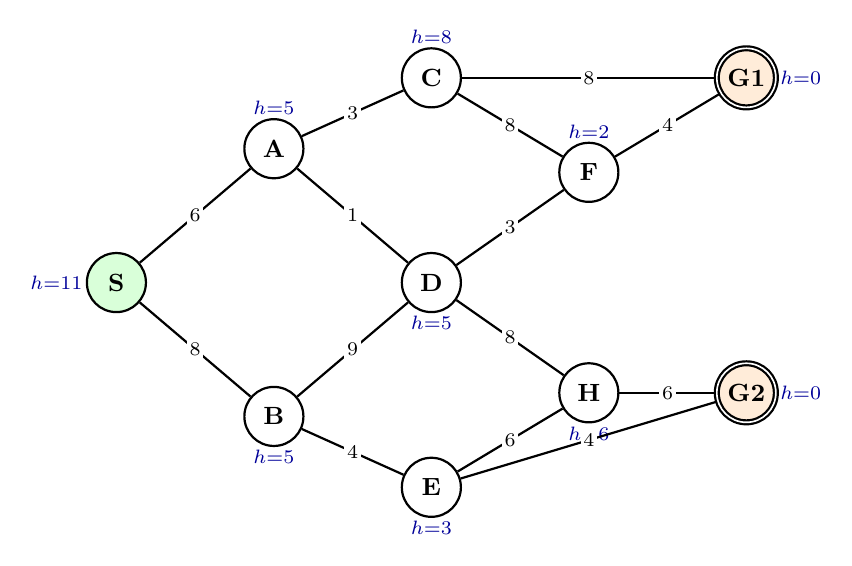
\begin{tikzpicture}[scale=1.0, every node/.style={transform shape}, gn/.style={draw, thick, circle, minimum size=7.5mm, inner sep=0pt, font=\small\bfseries}, ec/.style={font=\scriptsize, fill=white, inner sep=1pt}]
\node[gn, fill=green!15, label={[font=\scriptsize, text=blue!60!black, inner sep=1pt]left:$h{=}11$}] (S) at (0.00,0.00) {S};
\node[gn, label={[font=\scriptsize, text=blue!60!black, inner sep=1pt]above:$h{=}5$}] (A) at (2.00,1.70) {A};
\node[gn, label={[font=\scriptsize, text=blue!60!black, inner sep=1pt]below:$h{=}5$}] (B) at (2.00,-1.70) {B};
\node[gn, label={[font=\scriptsize, text=blue!60!black, inner sep=1pt]above:$h{=}8$}] (C) at (4.00,2.60) {C};
\node[gn, label={[font=\scriptsize, text=blue!60!black, inner sep=1pt]below:$h{=}5$}] (D) at (4.00,0.00) {D};
\node[gn, label={[font=\scriptsize, text=blue!60!black, inner sep=1pt]below:$h{=}3$}] (E) at (4.00,-2.60) {E};
\node[gn, label={[font=\scriptsize, text=blue!60!black, inner sep=1pt]above:$h{=}2$}] (F) at (6.00,1.40) {F};
\node[gn, label={[font=\scriptsize, text=blue!60!black, inner sep=1pt]below:$h{=}6$}] (H) at (6.00,-1.40) {H};
\node[gn, double, fill=orange!15, label={[font=\scriptsize, text=blue!60!black, inner sep=1pt]right:$h{=}0$}] (G1) at (8.00,2.60) {G1};
\node[gn, double, fill=orange!15, label={[font=\scriptsize, text=blue!60!black, inner sep=1pt]right:$h{=}0$}] (G2) at (8.00,-1.40) {G2};
\draw[thick] (S) to[] node[ec, midway]{6} (A);
\draw[thick] (S) to[] node[ec, midway]{8} (B);
\draw[thick] (A) to[] node[ec, midway]{3} (C);
\draw[thick] (A) to[] node[ec, midway]{1} (D);
\draw[thick] (B) to[] node[ec, midway]{9} (D);
\draw[thick] (B) to[] node[ec, midway]{4} (E);
\draw[thick] (C) to[] node[ec, midway]{8} (F);
\draw[thick] (C) to[] node[ec, midway]{8} (G1);
\draw[thick] (D) to[] node[ec, midway]{3} (F);
\draw[thick] (D) to[] node[ec, midway]{8} (H);
\draw[thick] (E) to[] node[ec, midway]{6} (H);
\draw[thick] (F) to[] node[ec, midway]{4} (G1);
\draw[thick] (H) to[] node[ec, midway]{6} (G2);
\draw[thick] (E) to[] node[ec, midway]{4} (G2);
\end{tikzpicture}
\end{adjustbox}
\end{center}For each search strategy, (a) list, in order, the states \textbf{expanded}, (b) give the path found and (c) give the final content of the frontier (a state is expanded when it is removed from the frontier). Conventions: BFS, DFS and greedy best-first search test a state for the goal when it is \emph{generated} (so the goal is not expanded); UCS and A* test it when it is \emph{removed} from the frontier (graph search; a cheaper path to a frontier state replaces its entry). DFS avoids loops by remembering the states on the current path only. The path returned will not be accepted if the list of expanded states is wrong.

\begin{solbox}
\begin{center}\small\begin{tabularx}{\linewidth}{|>{\raggedright}p{2.6cm}|>{\raggedright}X|>{\raggedright}p{3.6cm}|>{\raggedright\arraybackslash}p{2.6cm}|}\hline
\textbf{Algorithm} & \textbf{List of expanded states} & \textbf{Path returned} & \textbf{Final frontier}\\ \hline
Breadth-first search & \textcolor{blue!60!black}{S A B C} & \textcolor{blue!60!black}{S A C G1} (cost 17) & \textcolor{blue!60!black}{$\{$ D, E, F $\}$}\\ \hline
Uniform-cost search & \textcolor{blue!60!black}{S A D B C F E G1} & \textcolor{blue!60!black}{S A D F G1} (cost 14) & \textcolor{blue!60!black}{$\{$ H, G2 $\}$}\\ \hline
Depth-first search & \textcolor{blue!60!black}{S A C} & \textcolor{blue!60!black}{S A C G1} (cost 17) & \textcolor{blue!60!black}{(not asked)}\\ \hline
Greedy best-first search & \textcolor{blue!60!black}{S A B E} & \textcolor{blue!60!black}{S B E G2} (cost 16) & \textcolor{blue!60!black}{$\{$ D, C $\}$}\\ \hline
Graph-search A* & \textcolor{blue!60!black}{S A D F B G1} & \textcolor{blue!60!black}{S A D F G1} (cost 14) & \textcolor{blue!60!black}{$\{$ E, C, H $\}$}\\ \hline
\end{tabularx}\end{center}\textbf{BFS} (queue after each expansion):\begin{center}\small\begin{tabularx}{\linewidth}{c c >{\raggedright\arraybackslash}X}\toprule
Step & Expanded & Queue (front $\rightarrow$ back) after the expansion \\ \midrule
1 & S & A, B \\
2 & A & B, C, D \\
3 & B & C, D, E \\
4 & C & generates goal \textbf{G1} $\Rightarrow$ stop; frontier: D, E, F \\
\bottomrule\end{tabularx}\end{center}\textbf{DFS} (stack after each expansion):\begin{center}\small\begin{tabularx}{\linewidth}{c c >{\raggedright\arraybackslash}X}\toprule
Step & Expanded & Stack (top $\rightarrow$ bottom) after the expansion \\ \midrule
1 & S & A, B \\
2 & A & C, D, B \\
3 & C & generates goal \textbf{G1} $\Rightarrow$ stop; frontier: D, B \\
\bottomrule\end{tabularx}\end{center}\textbf{UCS:}\begin{center}\small\begin{tabularx}{\linewidth}{c l >{\raggedright\arraybackslash}X}\toprule
Step & Expanded & Frontier after the expansion, in priority order (subscript $=g(n)$) \\ \midrule
1 & S$_{0}$ & A$_{6}$, B$_{8}$ \\
2 & A$_{6}$ & D$_{7}$, B$_{8}$, C$_{9}$ \\
3 & D$_{7}$ & B$_{8}$, C$_{9}$, F$_{10}$, H$_{15}$ \\
4 & B$_{8}$ & C$_{9}$, F$_{10}$, E$_{12}$, H$_{15}$ \\
5 & C$_{9}$ & F$_{10}$, E$_{12}$, H$_{15}$, G1$_{17}$ \\
6 & F$_{10}$ & E$_{12}$, G1$_{14}$, H$_{15}$ \\
7 & E$_{12}$ & G1$_{14}$, H$_{15}$, G2$_{16}$ \\
8 & G1$_{14}$ & \textit{goal removed from the frontier -- stop} \\
\bottomrule\end{tabularx}\end{center}\textbf{Greedy best-first:}\begin{center}\small\begin{tabularx}{\linewidth}{c l >{\raggedright\arraybackslash}X}\toprule
Step & Expanded & Frontier after the expansion, in priority order (subscript $=h(n)$) \\ \midrule
1 & S$_{11}$ & A$_{5}$, B$_{5}$ \\
2 & A$_{5}$ & B$_{5}$, D$_{5}$, C$_{8}$ \\
3 & B$_{5}$ & E$_{3}$, D$_{5}$, C$_{8}$ \\
4 & E$_{3}$ & generates goal \textbf{G2} $\Rightarrow$ stop; frontier: D$_{5}$, C$_{8}$ \\
\bottomrule\end{tabularx}\end{center}\textbf{A*:}\begin{center}\small\begin{tabularx}{\linewidth}{c l >{\raggedright\arraybackslash}X}\toprule
Step & Expanded & Frontier after the expansion, in priority order (subscript $=g+h=f$) \\ \midrule
1 & S$_{0+11=11}$ & A$_{6+5=11}$, B$_{8+5=13}$ \\
2 & A$_{6+5=11}$ & D$_{7+5=12}$, B$_{8+5=13}$, C$_{9+8=17}$ \\
3 & D$_{7+5=12}$ & F$_{10+2=12}$, B$_{8+5=13}$, C$_{9+8=17}$, H$_{15+6=21}$ \\
4 & F$_{10+2=12}$ & B$_{8+5=13}$, G1$_{14+0=14}$, C$_{9+8=17}$, H$_{15+6=21}$ \\
5 & B$_{8+5=13}$ & G1$_{14+0=14}$, E$_{12+3=15}$, C$_{9+8=17}$, H$_{15+6=21}$ \\
6 & G1$_{14+0=14}$ & \textit{goal removed from the frontier -- stop} \\
\bottomrule\end{tabularx}\end{center}
\end{solbox}
\subq{(d)}With several goals, what must an admissible heuristic estimate? Is $h$ admissible and consistent?
\begin{solbox}
The cost to the \emph{nearest} goal. $h^*$: S$=14$, A$=8$, B$=8$, C$=8$, D$=7$, E$=4$, F$=4$, H$=6$, G1$=0$, G2$=0$; $h\le h^*$ (admissible) and $h(u)\le c(u,v)+h(v)$ on every edge (consistent).
\end{solbox}
\subq{(e)}Which goal does each strategy reach? Why does greedy best-first search end at a different goal from A*?
\begin{solbox}
BFS$\to$G1, UCS$\to$G1, DFS$\to$G1, GBFS$\to$G2, A*$\to$G1. GBFS only follows $h$: after the tie $A/B$ ($h=5$) and then $B/D$ (alphabetical), it expands $B$, whose child $E$ leads straight to $G_2$ (cost 16). A* also counts the cost already paid and finds the cheaper route to $G_1$ (cost 14).
\end{solbox}
\question{3}Consider the 8-puzzle. Apply \emph{steepest-descent hill climbing} with the Manhattan-distance heuristic $h$ to the following pair of initial and goal states.\begin{center}Initial state\quad \begin{tabular}{|c|c|c|}\hline 1 & 2 & 5\\\hline 3 & -- & 4\\\hline 6 & 7 & 8\\\hline\end{tabular}\qquad\qquad Goal state\quad \begin{tabular}{|c|c|c|}\hline -- & 1 & 2\\\hline 3 & 4 & 5\\\hline 6 & 7 & 8\\\hline\end{tabular}\end{center}Your work should: draw the search tree including all successors of every expanded state (moves of the blank in the order Up, Down, Left, Right; do not regenerate the parent state), write the heuristic value of every node, and mark the path found.
\par\smallskip\noindent 
\begin{solbox}
\begin{center}
\begin{adjustbox}{max width=\linewidth}
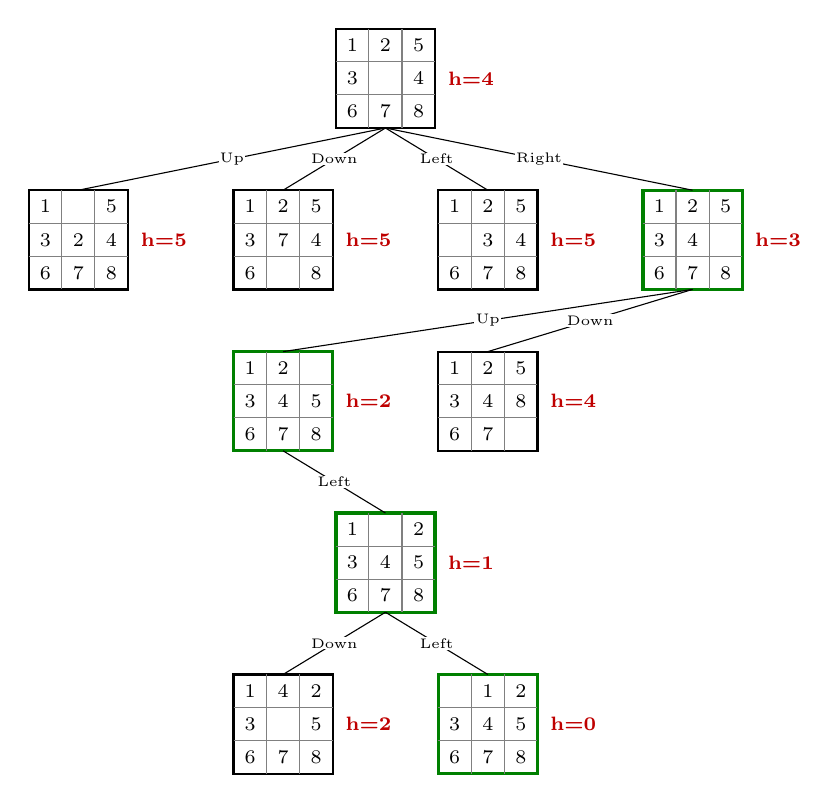
\begin{tikzpicture}
\draw[thick] (-0.63,0.00) rectangle (0.63,-1.26);
\draw[black!50] (-0.21,0.00) -- (-0.21,-1.26);
\draw[black!50] (-0.63,-0.42) -- (0.63,-0.42);
\draw[black!50] (0.21,0.00) -- (0.21,-1.26);
\draw[black!50] (-0.63,-0.84) -- (0.63,-0.84);
\node[font=\scriptsize] at (-0.42,-0.21) {1};
\node[font=\scriptsize] at (0.00,-0.21) {2};
\node[font=\scriptsize] at (0.42,-0.21) {5};
\node[font=\scriptsize] at (-0.42,-0.63) {3};
\node[font=\scriptsize] at (0.42,-0.63) {4};
\node[font=\scriptsize] at (-0.42,-1.05) {6};
\node[font=\scriptsize] at (0.00,-1.05) {7};
\node[font=\scriptsize] at (0.42,-1.05) {8};
\coordinate (r0-top) at (0.00,0.00);
\coordinate (r0-bot) at (0.00,-1.26);
\node[font=\scriptsize\bfseries, text=red!75!black, anchor=west] at (0.67,-0.63) {h=4};
\draw[thick] (-4.53,-2.05) rectangle (-3.27,-3.31);
\draw[black!50] (-4.11,-2.05) -- (-4.11,-3.31);
\draw[black!50] (-4.53,-2.47) -- (-3.27,-2.47);
\draw[black!50] (-3.69,-2.05) -- (-3.69,-3.31);
\draw[black!50] (-4.53,-2.89) -- (-3.27,-2.89);
\node[font=\scriptsize] at (-4.32,-2.26) {1};
\node[font=\scriptsize] at (-3.48,-2.26) {5};
\node[font=\scriptsize] at (-4.32,-2.68) {3};
\node[font=\scriptsize] at (-3.90,-2.68) {2};
\node[font=\scriptsize] at (-3.48,-2.68) {4};
\node[font=\scriptsize] at (-4.32,-3.10) {6};
\node[font=\scriptsize] at (-3.90,-3.10) {7};
\node[font=\scriptsize] at (-3.48,-3.10) {8};
\coordinate (b0_0-top) at (-3.90,-2.05);
\coordinate (b0_0-bot) at (-3.90,-3.31);
\node[font=\scriptsize\bfseries, text=red!75!black, anchor=west] at (-3.23,-2.68) {h=5};
\draw (r0-bot) -- node[font=\tiny, fill=white, inner sep=0.5pt]{Up} (b0_0-top);
\draw[thick] (-1.93,-2.05) rectangle (-0.67,-3.31);
\draw[black!50] (-1.51,-2.05) -- (-1.51,-3.31);
\draw[black!50] (-1.93,-2.47) -- (-0.67,-2.47);
\draw[black!50] (-1.09,-2.05) -- (-1.09,-3.31);
\draw[black!50] (-1.93,-2.89) -- (-0.67,-2.89);
\node[font=\scriptsize] at (-1.72,-2.26) {1};
\node[font=\scriptsize] at (-1.30,-2.26) {2};
\node[font=\scriptsize] at (-0.88,-2.26) {5};
\node[font=\scriptsize] at (-1.72,-2.68) {3};
\node[font=\scriptsize] at (-1.30,-2.68) {7};
\node[font=\scriptsize] at (-0.88,-2.68) {4};
\node[font=\scriptsize] at (-1.72,-3.10) {6};
\node[font=\scriptsize] at (-0.88,-3.10) {8};
\coordinate (b0_1-top) at (-1.30,-2.05);
\coordinate (b0_1-bot) at (-1.30,-3.31);
\node[font=\scriptsize\bfseries, text=red!75!black, anchor=west] at (-0.63,-2.68) {h=5};
\draw (r0-bot) -- node[font=\tiny, fill=white, inner sep=0.5pt]{Down} (b0_1-top);
\draw[thick] (0.67,-2.05) rectangle (1.93,-3.31);
\draw[black!50] (1.09,-2.05) -- (1.09,-3.31);
\draw[black!50] (0.67,-2.47) -- (1.93,-2.47);
\draw[black!50] (1.51,-2.05) -- (1.51,-3.31);
\draw[black!50] (0.67,-2.89) -- (1.93,-2.89);
\node[font=\scriptsize] at (0.88,-2.26) {1};
\node[font=\scriptsize] at (1.30,-2.26) {2};
\node[font=\scriptsize] at (1.72,-2.26) {5};
\node[font=\scriptsize] at (1.30,-2.68) {3};
\node[font=\scriptsize] at (1.72,-2.68) {4};
\node[font=\scriptsize] at (0.88,-3.10) {6};
\node[font=\scriptsize] at (1.30,-3.10) {7};
\node[font=\scriptsize] at (1.72,-3.10) {8};
\coordinate (b0_2-top) at (1.30,-2.05);
\coordinate (b0_2-bot) at (1.30,-3.31);
\node[font=\scriptsize\bfseries, text=red!75!black, anchor=west] at (1.97,-2.68) {h=5};
\draw (r0-bot) -- node[font=\tiny, fill=white, inner sep=0.5pt]{Left} (b0_2-top);
\draw[very thick, draw=green!50!black] (3.27,-2.05) rectangle (4.53,-3.31);
\draw[black!50] (3.69,-2.05) -- (3.69,-3.31);
\draw[black!50] (3.27,-2.47) -- (4.53,-2.47);
\draw[black!50] (4.11,-2.05) -- (4.11,-3.31);
\draw[black!50] (3.27,-2.89) -- (4.53,-2.89);
\node[font=\scriptsize] at (3.48,-2.26) {1};
\node[font=\scriptsize] at (3.90,-2.26) {2};
\node[font=\scriptsize] at (4.32,-2.26) {5};
\node[font=\scriptsize] at (3.48,-2.68) {3};
\node[font=\scriptsize] at (3.90,-2.68) {4};
\node[font=\scriptsize] at (3.48,-3.10) {6};
\node[font=\scriptsize] at (3.90,-3.10) {7};
\node[font=\scriptsize] at (4.32,-3.10) {8};
\coordinate (b0_3-top) at (3.90,-2.05);
\coordinate (b0_3-bot) at (3.90,-3.31);
\node[font=\scriptsize\bfseries, text=red!75!black, anchor=west] at (4.57,-2.68) {h=3};
\draw (r0-bot) -- node[font=\tiny, fill=white, inner sep=0.5pt]{Right} (b0_3-top);
\draw[very thick, draw=green!50!black] (-1.93,-4.10) rectangle (-0.67,-5.36);
\draw[black!50] (-1.51,-4.10) -- (-1.51,-5.36);
\draw[black!50] (-1.93,-4.52) -- (-0.67,-4.52);
\draw[black!50] (-1.09,-4.10) -- (-1.09,-5.36);
\draw[black!50] (-1.93,-4.94) -- (-0.67,-4.94);
\node[font=\scriptsize] at (-1.72,-4.31) {1};
\node[font=\scriptsize] at (-1.30,-4.31) {2};
\node[font=\scriptsize] at (-1.72,-4.73) {3};
\node[font=\scriptsize] at (-1.30,-4.73) {4};
\node[font=\scriptsize] at (-0.88,-4.73) {5};
\node[font=\scriptsize] at (-1.72,-5.15) {6};
\node[font=\scriptsize] at (-1.30,-5.15) {7};
\node[font=\scriptsize] at (-0.88,-5.15) {8};
\coordinate (b1_0-top) at (-1.30,-4.10);
\coordinate (b1_0-bot) at (-1.30,-5.36);
\node[font=\scriptsize\bfseries, text=red!75!black, anchor=west] at (-0.63,-4.73) {h=2};
\draw (b0_3-bot) -- node[font=\tiny, fill=white, inner sep=0.5pt]{Up} (b1_0-top);
\draw[thick] (0.67,-4.10) rectangle (1.93,-5.36);
\draw[black!50] (1.09,-4.10) -- (1.09,-5.36);
\draw[black!50] (0.67,-4.52) -- (1.93,-4.52);
\draw[black!50] (1.51,-4.10) -- (1.51,-5.36);
\draw[black!50] (0.67,-4.94) -- (1.93,-4.94);
\node[font=\scriptsize] at (0.88,-4.31) {1};
\node[font=\scriptsize] at (1.30,-4.31) {2};
\node[font=\scriptsize] at (1.72,-4.31) {5};
\node[font=\scriptsize] at (0.88,-4.73) {3};
\node[font=\scriptsize] at (1.30,-4.73) {4};
\node[font=\scriptsize] at (1.72,-4.73) {8};
\node[font=\scriptsize] at (0.88,-5.15) {6};
\node[font=\scriptsize] at (1.30,-5.15) {7};
\coordinate (b1_1-top) at (1.30,-4.10);
\coordinate (b1_1-bot) at (1.30,-5.36);
\node[font=\scriptsize\bfseries, text=red!75!black, anchor=west] at (1.97,-4.73) {h=4};
\draw (b0_3-bot) -- node[font=\tiny, fill=white, inner sep=0.5pt]{Down} (b1_1-top);
\draw[very thick, draw=green!50!black] (-0.63,-6.15) rectangle (0.63,-7.41);
\draw[black!50] (-0.21,-6.15) -- (-0.21,-7.41);
\draw[black!50] (-0.63,-6.57) -- (0.63,-6.57);
\draw[black!50] (0.21,-6.15) -- (0.21,-7.41);
\draw[black!50] (-0.63,-6.99) -- (0.63,-6.99);
\node[font=\scriptsize] at (-0.42,-6.36) {1};
\node[font=\scriptsize] at (0.42,-6.36) {2};
\node[font=\scriptsize] at (-0.42,-6.78) {3};
\node[font=\scriptsize] at (0.00,-6.78) {4};
\node[font=\scriptsize] at (0.42,-6.78) {5};
\node[font=\scriptsize] at (-0.42,-7.20) {6};
\node[font=\scriptsize] at (0.00,-7.20) {7};
\node[font=\scriptsize] at (0.42,-7.20) {8};
\coordinate (b2_0-top) at (0.00,-6.15);
\coordinate (b2_0-bot) at (0.00,-7.41);
\node[font=\scriptsize\bfseries, text=red!75!black, anchor=west] at (0.67,-6.78) {h=1};
\draw (b1_0-bot) -- node[font=\tiny, fill=white, inner sep=0.5pt]{Left} (b2_0-top);
\draw[thick] (-1.93,-8.20) rectangle (-0.67,-9.46);
\draw[black!50] (-1.51,-8.20) -- (-1.51,-9.46);
\draw[black!50] (-1.93,-8.62) -- (-0.67,-8.62);
\draw[black!50] (-1.09,-8.20) -- (-1.09,-9.46);
\draw[black!50] (-1.93,-9.04) -- (-0.67,-9.04);
\node[font=\scriptsize] at (-1.72,-8.41) {1};
\node[font=\scriptsize] at (-1.30,-8.41) {4};
\node[font=\scriptsize] at (-0.88,-8.41) {2};
\node[font=\scriptsize] at (-1.72,-8.83) {3};
\node[font=\scriptsize] at (-0.88,-8.83) {5};
\node[font=\scriptsize] at (-1.72,-9.25) {6};
\node[font=\scriptsize] at (-1.30,-9.25) {7};
\node[font=\scriptsize] at (-0.88,-9.25) {8};
\coordinate (b3_0-top) at (-1.30,-8.20);
\coordinate (b3_0-bot) at (-1.30,-9.46);
\node[font=\scriptsize\bfseries, text=red!75!black, anchor=west] at (-0.63,-8.83) {h=2};
\draw (b2_0-bot) -- node[font=\tiny, fill=white, inner sep=0.5pt]{Down} (b3_0-top);
\draw[very thick, draw=green!50!black] (0.67,-8.20) rectangle (1.93,-9.46);
\draw[black!50] (1.09,-8.20) -- (1.09,-9.46);
\draw[black!50] (0.67,-8.62) -- (1.93,-8.62);
\draw[black!50] (1.51,-8.20) -- (1.51,-9.46);
\draw[black!50] (0.67,-9.04) -- (1.93,-9.04);
\node[font=\scriptsize] at (1.30,-8.41) {1};
\node[font=\scriptsize] at (1.72,-8.41) {2};
\node[font=\scriptsize] at (0.88,-8.83) {3};
\node[font=\scriptsize] at (1.30,-8.83) {4};
\node[font=\scriptsize] at (1.72,-8.83) {5};
\node[font=\scriptsize] at (0.88,-9.25) {6};
\node[font=\scriptsize] at (1.30,-9.25) {7};
\node[font=\scriptsize] at (1.72,-9.25) {8};
\coordinate (b3_1-top) at (1.30,-8.20);
\coordinate (b3_1-bot) at (1.30,-9.46);
\node[font=\scriptsize\bfseries, text=red!75!black, anchor=west] at (1.97,-8.83) {h=0};
\draw (b2_0-bot) -- node[font=\tiny, fill=white, inner sep=0.5pt]{Left} (b3_1-top);
\end{tikzpicture}
\end{adjustbox}
\end{center}Each level keeps the successor with the smallest $h$ (green). $h$ decreases 4$\to$3$\to$2$\to$1$\to$0 and the goal is reached after 4 moves: Right, Up, Left, Left.
\end{solbox}
\question{4}Consider the following game tree (MAX at the root).\begin{center}
\begin{adjustbox}{max width=\linewidth}
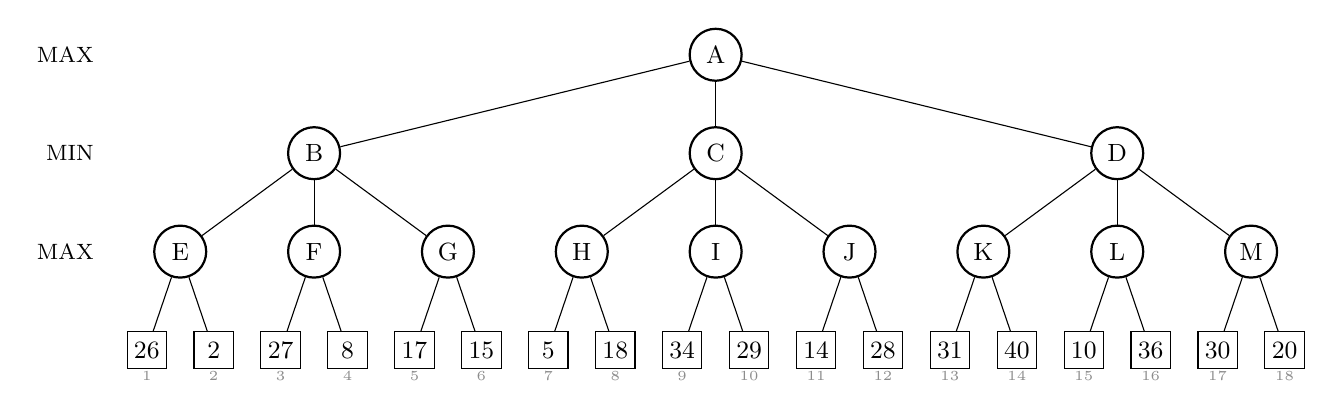
\begin{tikzpicture}[scale=1.0, every node/.style={transform shape}, gc/.style={draw, thick, circle, minimum size=6.6mm, inner sep=0pt, font=\small}, gl/.style={draw, rectangle, minimum width=5mm, minimum height=4.6mm, inner sep=1pt, font=\small}, gx/.style={draw=black!25, text=black!35}, val/.style={font=\footnotesize\bfseries, text=red!80!black, inner sep=1pt}]
\node[font=\footnotesize, anchor=east] at (-0.55,0.00) {MAX};
\node[font=\footnotesize, anchor=east] at (-0.55,-1.25) {MIN};
\node[font=\footnotesize, anchor=east] at (-0.55,-2.50) {MAX};
\node[gc] (n30) at (7.225,0.000) {A};
\node[gc] (n9) at (2.125,-1.250) {B};
\node[gc] (n2) at (0.425,-2.500) {E};
\node[gl, label={[font=\tiny, text=black!45, inner sep=1pt]below:1}] (n0) at (0.000,-3.750) {26};
\node[gl, label={[font=\tiny, text=black!45, inner sep=1pt]below:2}] (n1) at (0.850,-3.750) {2};
\node[gc] (n5) at (2.125,-2.500) {F};
\node[gl, label={[font=\tiny, text=black!45, inner sep=1pt]below:3}] (n3) at (1.700,-3.750) {27};
\node[gl, label={[font=\tiny, text=black!45, inner sep=1pt]below:4}] (n4) at (2.550,-3.750) {8};
\node[gc] (n8) at (3.825,-2.500) {G};
\node[gl, label={[font=\tiny, text=black!45, inner sep=1pt]below:5}] (n6) at (3.400,-3.750) {17};
\node[gl, label={[font=\tiny, text=black!45, inner sep=1pt]below:6}] (n7) at (4.250,-3.750) {15};
\node[gc] (n19) at (7.225,-1.250) {C};
\node[gc] (n12) at (5.525,-2.500) {H};
\node[gl, label={[font=\tiny, text=black!45, inner sep=1pt]below:7}] (n10) at (5.100,-3.750) {5};
\node[gl, label={[font=\tiny, text=black!45, inner sep=1pt]below:8}] (n11) at (5.950,-3.750) {18};
\node[gc] (n15) at (7.225,-2.500) {I};
\node[gl, label={[font=\tiny, text=black!45, inner sep=1pt]below:9}] (n13) at (6.800,-3.750) {34};
\node[gl, label={[font=\tiny, text=black!45, inner sep=1pt]below:10}] (n14) at (7.650,-3.750) {29};
\node[gc] (n18) at (8.925,-2.500) {J};
\node[gl, label={[font=\tiny, text=black!45, inner sep=1pt]below:11}] (n16) at (8.500,-3.750) {14};
\node[gl, label={[font=\tiny, text=black!45, inner sep=1pt]below:12}] (n17) at (9.350,-3.750) {28};
\node[gc] (n29) at (12.325,-1.250) {D};
\node[gc] (n22) at (10.625,-2.500) {K};
\node[gl, label={[font=\tiny, text=black!45, inner sep=1pt]below:13}] (n20) at (10.200,-3.750) {31};
\node[gl, label={[font=\tiny, text=black!45, inner sep=1pt]below:14}] (n21) at (11.050,-3.750) {40};
\node[gc] (n25) at (12.325,-2.500) {L};
\node[gl, label={[font=\tiny, text=black!45, inner sep=1pt]below:15}] (n23) at (11.900,-3.750) {10};
\node[gl, label={[font=\tiny, text=black!45, inner sep=1pt]below:16}] (n24) at (12.750,-3.750) {36};
\node[gc] (n28) at (14.025,-2.500) {M};
\node[gl, label={[font=\tiny, text=black!45, inner sep=1pt]below:17}] (n26) at (13.600,-3.750) {30};
\node[gl, label={[font=\tiny, text=black!45, inner sep=1pt]below:18}] (n27) at (14.450,-3.750) {20};
\draw (n30) -- (n9);
\draw (n30) -- (n19);
\draw (n30) -- (n29);
\draw (n9) -- (n2);
\draw (n9) -- (n5);
\draw (n9) -- (n8);
\draw (n2) -- (n0);
\draw (n2) -- (n1);
\draw (n5) -- (n3);
\draw (n5) -- (n4);
\draw (n8) -- (n6);
\draw (n8) -- (n7);
\draw (n19) -- (n12);
\draw (n19) -- (n15);
\draw (n19) -- (n18);
\draw (n12) -- (n10);
\draw (n12) -- (n11);
\draw (n15) -- (n13);
\draw (n15) -- (n14);
\draw (n18) -- (n16);
\draw (n18) -- (n17);
\draw (n29) -- (n22);
\draw (n29) -- (n25);
\draw (n29) -- (n28);
\draw (n22) -- (n20);
\draw (n22) -- (n21);
\draw (n25) -- (n23);
\draw (n25) -- (n24);
\draw (n28) -- (n26);
\draw (n28) -- (n27);
\end{tikzpicture}
\end{adjustbox}
\end{center}
\subq{(a)}Compute the final backed-up value of every node using the minimax algorithm (no alpha-beta pruning at this step). Which move should MAX make at the root?
\begin{solbox}
\begin{center}\small \begin{tabular}{|l|c|c|c|c|c|c|c|c|c|c|c|c|c|}\hline
\textbf{Node} & \textbf{A} & \textbf{B} & \textbf{C} & \textbf{D} & \textbf{E} & \textbf{F} & \textbf{G} & \textbf{H} & \textbf{I} & \textbf{J} & \textbf{K} & \textbf{L} & \textbf{M}\\ \hline
Minimax & \textcolor{blue!60!black}{30} & \textcolor{blue!60!black}{17} & \textcolor{blue!60!black}{18} & \textcolor{blue!60!black}{30} & \textcolor{blue!60!black}{26} & \textcolor{blue!60!black}{27} & \textcolor{blue!60!black}{17} & \textcolor{blue!60!black}{18} & \textcolor{blue!60!black}{34} & \textcolor{blue!60!black}{28} & \textcolor{blue!60!black}{40} & \textcolor{blue!60!black}{36} & \textcolor{blue!60!black}{30}\\[1.5mm] \hline
\end{tabular}\end{center}\begin{center}
\begin{adjustbox}{max width=\linewidth}
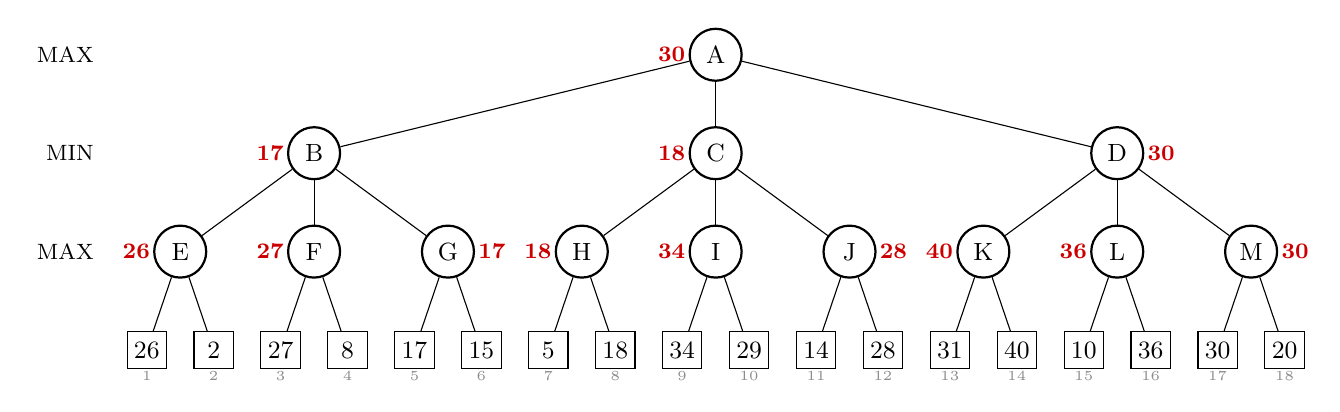
\begin{tikzpicture}[scale=1.0, every node/.style={transform shape}, gc/.style={draw, thick, circle, minimum size=6.6mm, inner sep=0pt, font=\small}, gl/.style={draw, rectangle, minimum width=5mm, minimum height=4.6mm, inner sep=1pt, font=\small}, gx/.style={draw=black!25, text=black!35}, val/.style={font=\footnotesize\bfseries, text=red!80!black, inner sep=1pt}]
\node[font=\footnotesize, anchor=east] at (-0.55,0.00) {MAX};
\node[font=\footnotesize, anchor=east] at (-0.55,-1.25) {MIN};
\node[font=\footnotesize, anchor=east] at (-0.55,-2.50) {MAX};
\node[gc, label={[val]left:30}] (n30) at (7.225,0.000) {A};
\node[gc, label={[val]left:17}] (n9) at (2.125,-1.250) {B};
\node[gc, label={[val]left:26}] (n2) at (0.425,-2.500) {E};
\node[gl, label={[font=\tiny, text=black!45, inner sep=1pt]below:1}] (n0) at (0.000,-3.750) {26};
\node[gl, label={[font=\tiny, text=black!45, inner sep=1pt]below:2}] (n1) at (0.850,-3.750) {2};
\node[gc, label={[val]left:27}] (n5) at (2.125,-2.500) {F};
\node[gl, label={[font=\tiny, text=black!45, inner sep=1pt]below:3}] (n3) at (1.700,-3.750) {27};
\node[gl, label={[font=\tiny, text=black!45, inner sep=1pt]below:4}] (n4) at (2.550,-3.750) {8};
\node[gc, label={[val]right:17}] (n8) at (3.825,-2.500) {G};
\node[gl, label={[font=\tiny, text=black!45, inner sep=1pt]below:5}] (n6) at (3.400,-3.750) {17};
\node[gl, label={[font=\tiny, text=black!45, inner sep=1pt]below:6}] (n7) at (4.250,-3.750) {15};
\node[gc, label={[val]left:18}] (n19) at (7.225,-1.250) {C};
\node[gc, label={[val]left:18}] (n12) at (5.525,-2.500) {H};
\node[gl, label={[font=\tiny, text=black!45, inner sep=1pt]below:7}] (n10) at (5.100,-3.750) {5};
\node[gl, label={[font=\tiny, text=black!45, inner sep=1pt]below:8}] (n11) at (5.950,-3.750) {18};
\node[gc, label={[val]left:34}] (n15) at (7.225,-2.500) {I};
\node[gl, label={[font=\tiny, text=black!45, inner sep=1pt]below:9}] (n13) at (6.800,-3.750) {34};
\node[gl, label={[font=\tiny, text=black!45, inner sep=1pt]below:10}] (n14) at (7.650,-3.750) {29};
\node[gc, label={[val]right:28}] (n18) at (8.925,-2.500) {J};
\node[gl, label={[font=\tiny, text=black!45, inner sep=1pt]below:11}] (n16) at (8.500,-3.750) {14};
\node[gl, label={[font=\tiny, text=black!45, inner sep=1pt]below:12}] (n17) at (9.350,-3.750) {28};
\node[gc, label={[val]right:30}] (n29) at (12.325,-1.250) {D};
\node[gc, label={[val]left:40}] (n22) at (10.625,-2.500) {K};
\node[gl, label={[font=\tiny, text=black!45, inner sep=1pt]below:13}] (n20) at (10.200,-3.750) {31};
\node[gl, label={[font=\tiny, text=black!45, inner sep=1pt]below:14}] (n21) at (11.050,-3.750) {40};
\node[gc, label={[val]left:36}] (n25) at (12.325,-2.500) {L};
\node[gl, label={[font=\tiny, text=black!45, inner sep=1pt]below:15}] (n23) at (11.900,-3.750) {10};
\node[gl, label={[font=\tiny, text=black!45, inner sep=1pt]below:16}] (n24) at (12.750,-3.750) {36};
\node[gc, label={[val]right:30}] (n28) at (14.025,-2.500) {M};
\node[gl, label={[font=\tiny, text=black!45, inner sep=1pt]below:17}] (n26) at (13.600,-3.750) {30};
\node[gl, label={[font=\tiny, text=black!45, inner sep=1pt]below:18}] (n27) at (14.450,-3.750) {20};
\draw (n30) -- (n9);
\draw (n30) -- (n19);
\draw (n30) -- (n29);
\draw (n9) -- (n2);
\draw (n9) -- (n5);
\draw (n9) -- (n8);
\draw (n2) -- (n0);
\draw (n2) -- (n1);
\draw (n5) -- (n3);
\draw (n5) -- (n4);
\draw (n8) -- (n6);
\draw (n8) -- (n7);
\draw (n19) -- (n12);
\draw (n19) -- (n15);
\draw (n19) -- (n18);
\draw (n12) -- (n10);
\draw (n12) -- (n11);
\draw (n15) -- (n13);
\draw (n15) -- (n14);
\draw (n18) -- (n16);
\draw (n18) -- (n17);
\draw (n29) -- (n22);
\draw (n29) -- (n25);
\draw (n29) -- (n28);
\draw (n22) -- (n20);
\draw (n22) -- (n21);
\draw (n25) -- (n23);
\draw (n25) -- (n24);
\draw (n28) -- (n26);
\draw (n28) -- (n27);
\end{tikzpicture}
\end{adjustbox}
\end{center}Root value $=30$; MAX moves to \textbf{D}.
\end{solbox}
\subq{(b)}Run alpha-beta pruning (children visited left to right). Give the value computed at every node (mark \textbf{X} if the node is never visited), cross out the pruned branches on the tree and briefly explain each case.
\begin{solbox}
\begin{center}\small \begin{tabular}{|l|c|c|c|c|c|c|c|c|c|c|c|c|c|}\hline
\textbf{Node} & \textbf{A} & \textbf{B} & \textbf{C} & \textbf{D} & \textbf{E} & \textbf{F} & \textbf{G} & \textbf{H} & \textbf{I} & \textbf{J} & \textbf{K} & \textbf{L} & \textbf{M}\\ \hline
$\alpha$-$\beta$ & \textcolor{blue!60!black}{$30$} & \textcolor{blue!60!black}{$17$} & \textcolor{blue!60!black}{$18$} & \textcolor{blue!60!black}{$30$} & \textcolor{blue!60!black}{$26$} & \textcolor{blue!60!black}{$\ge 27$} & \textcolor{blue!60!black}{$17$} & \textcolor{blue!60!black}{$18$} & \textcolor{blue!60!black}{$\ge 34$} & \textcolor{blue!60!black}{$28$} & \textcolor{blue!60!black}{$40$} & \textcolor{blue!60!black}{$36$} & \textcolor{blue!60!black}{$30$}\\[1.5mm] \hline
\end{tabular}\end{center}($\le v$ / $\ge v$: the node was cut off, so only this bound is known; writing the returned number $v$ is also accepted.)\begin{center}
\begin{adjustbox}{max width=\linewidth}
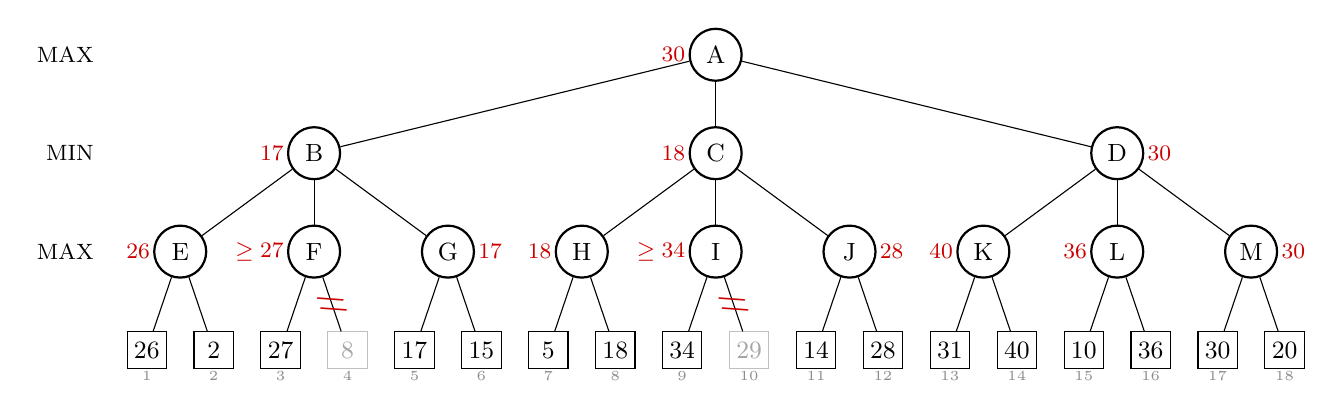
\begin{tikzpicture}[scale=1.0, every node/.style={transform shape}, gc/.style={draw, thick, circle, minimum size=6.6mm, inner sep=0pt, font=\small}, gl/.style={draw, rectangle, minimum width=5mm, minimum height=4.6mm, inner sep=1pt, font=\small}, gx/.style={draw=black!25, text=black!35}, val/.style={font=\footnotesize\bfseries, text=red!80!black, inner sep=1pt}]
\node[font=\footnotesize, anchor=east] at (-0.55,0.00) {MAX};
\node[font=\footnotesize, anchor=east] at (-0.55,-1.25) {MIN};
\node[font=\footnotesize, anchor=east] at (-0.55,-2.50) {MAX};
\node[gc, label={[val]left:$30$}] (n30) at (7.225,0.000) {A};
\node[gc, label={[val]left:$17$}] (n9) at (2.125,-1.250) {B};
\node[gc, label={[val]left:$26$}] (n2) at (0.425,-2.500) {E};
\node[gl, label={[font=\tiny, text=black!45, inner sep=1pt]below:1}] (n0) at (0.000,-3.750) {26};
\node[gl, label={[font=\tiny, text=black!45, inner sep=1pt]below:2}] (n1) at (0.850,-3.750) {2};
\node[gc, label={[val]left:$\ge27$}] (n5) at (2.125,-2.500) {F};
\node[gl, label={[font=\tiny, text=black!45, inner sep=1pt]below:3}] (n3) at (1.700,-3.750) {27};
\node[gl, gx, label={[font=\tiny, text=black!45, inner sep=1pt]below:4}] (n4) at (2.550,-3.750) {8};
\node[gc, label={[val]right:$17$}] (n8) at (3.825,-2.500) {G};
\node[gl, label={[font=\tiny, text=black!45, inner sep=1pt]below:5}] (n6) at (3.400,-3.750) {17};
\node[gl, label={[font=\tiny, text=black!45, inner sep=1pt]below:6}] (n7) at (4.250,-3.750) {15};
\node[gc, label={[val]left:$18$}] (n19) at (7.225,-1.250) {C};
\node[gc, label={[val]left:$18$}] (n12) at (5.525,-2.500) {H};
\node[gl, label={[font=\tiny, text=black!45, inner sep=1pt]below:7}] (n10) at (5.100,-3.750) {5};
\node[gl, label={[font=\tiny, text=black!45, inner sep=1pt]below:8}] (n11) at (5.950,-3.750) {18};
\node[gc, label={[val]left:$\ge34$}] (n15) at (7.225,-2.500) {I};
\node[gl, label={[font=\tiny, text=black!45, inner sep=1pt]below:9}] (n13) at (6.800,-3.750) {34};
\node[gl, gx, label={[font=\tiny, text=black!45, inner sep=1pt]below:10}] (n14) at (7.650,-3.750) {29};
\node[gc, label={[val]right:$28$}] (n18) at (8.925,-2.500) {J};
\node[gl, label={[font=\tiny, text=black!45, inner sep=1pt]below:11}] (n16) at (8.500,-3.750) {14};
\node[gl, label={[font=\tiny, text=black!45, inner sep=1pt]below:12}] (n17) at (9.350,-3.750) {28};
\node[gc, label={[val]right:$30$}] (n29) at (12.325,-1.250) {D};
\node[gc, label={[val]left:$40$}] (n22) at (10.625,-2.500) {K};
\node[gl, label={[font=\tiny, text=black!45, inner sep=1pt]below:13}] (n20) at (10.200,-3.750) {31};
\node[gl, label={[font=\tiny, text=black!45, inner sep=1pt]below:14}] (n21) at (11.050,-3.750) {40};
\node[gc, label={[val]left:$36$}] (n25) at (12.325,-2.500) {L};
\node[gl, label={[font=\tiny, text=black!45, inner sep=1pt]below:15}] (n23) at (11.900,-3.750) {10};
\node[gl, label={[font=\tiny, text=black!45, inner sep=1pt]below:16}] (n24) at (12.750,-3.750) {36};
\node[gc, label={[val]right:$30$}] (n28) at (14.025,-2.500) {M};
\node[gl, label={[font=\tiny, text=black!45, inner sep=1pt]below:17}] (n26) at (13.600,-3.750) {30};
\node[gl, label={[font=\tiny, text=black!45, inner sep=1pt]below:18}] (n27) at (14.450,-3.750) {20};
\draw (n30) -- (n9);
\draw (n30) -- (n19);
\draw (n30) -- (n29);
\draw (n9) -- (n2);
\draw (n9) -- (n5);
\draw (n9) -- (n8);
\draw (n2) -- (n0);
\draw (n2) -- (n1);
\draw (n5) -- (n3);
\draw (n5) -- (n4) node[midway, sloped, text=red!80!black, font=\small\bfseries, inner sep=0pt]{/\!/};
\draw (n8) -- (n6);
\draw (n8) -- (n7);
\draw (n19) -- (n12);
\draw (n19) -- (n15);
\draw (n19) -- (n18);
\draw (n12) -- (n10);
\draw (n12) -- (n11);
\draw (n15) -- (n13);
\draw (n15) -- (n14) node[midway, sloped, text=red!80!black, font=\small\bfseries, inner sep=0pt]{/\!/};
\draw (n18) -- (n16);
\draw (n18) -- (n17);
\draw (n29) -- (n22);
\draw (n29) -- (n25);
\draw (n29) -- (n28);
\draw (n22) -- (n20);
\draw (n22) -- (n21);
\draw (n25) -- (n23);
\draw (n25) -- (n24);
\draw (n28) -- (n26);
\draw (n28) -- (n27);
\end{tikzpicture}
\end{adjustbox}
\end{center}$\alpha$ and $\beta$ at every visited node:\begin{center}\small\begin{tabular}{c c c c c}\toprule Node & Type & On entry & When it returns & Value returned\\\midrule A & MAX & $\alpha=-\infty,\ \beta=+\infty$ & $\alpha=30,\ \beta=+\infty$ & $30$ \\
B & MIN & $\alpha=-\infty,\ \beta=+\infty$ & $\alpha=-\infty,\ \beta=17$ & $17$ \\
E & MAX & $\alpha=-\infty,\ \beta=+\infty$ & $\alpha=26,\ \beta=+\infty$ & $26$ \\
F & MAX & $\alpha=-\infty,\ \beta=26$ & $\alpha=27,\ \beta=26$ & $\ge 27$ \\
G & MAX & $\alpha=-\infty,\ \beta=26$ & $\alpha=17,\ \beta=26$ & $17$ \\
C & MIN & $\alpha=17,\ \beta=+\infty$ & $\alpha=17,\ \beta=18$ & $18$ \\
H & MAX & $\alpha=17,\ \beta=+\infty$ & $\alpha=18,\ \beta=+\infty$ & $18$ \\
I & MAX & $\alpha=17,\ \beta=18$ & $\alpha=34,\ \beta=18$ & $\ge 34$ \\
J & MAX & $\alpha=17,\ \beta=18$ & $\alpha=28,\ \beta=18$ & $28$ \\
D & MIN & $\alpha=18,\ \beta=+\infty$ & $\alpha=18,\ \beta=30$ & $30$ \\
K & MAX & $\alpha=18,\ \beta=+\infty$ & $\alpha=40,\ \beta=+\infty$ & $40$ \\
L & MAX & $\alpha=18,\ \beta=40$ & $\alpha=36,\ \beta=40$ & $36$ \\
M & MAX & $\alpha=18,\ \beta=36$ & $\alpha=30,\ \beta=36$ & $30$ \\\bottomrule\end{tabular}\end{center}\begin{itemize}[leftmargin=1.5em,itemsep=1pt]
\item At MAX node \textbf{F}, after leaf \#3: $v=27 \ge \beta=26$ $\Rightarrow$ prune leaf \#4. (MIN at B already has an alternative worth $\beta=26$, so it will never let play reach F.)
\item At MAX node \textbf{I}, after leaf \#9: $v=34 \ge \beta=18$ $\Rightarrow$ prune leaf \#10. (MIN at C already has an alternative worth $\beta=18$, so it will never let play reach I.)
\end{itemize}Leaves evaluated: 16 of 18.
\end{solbox}
\subq{(c)}Run alpha-beta again, this time visiting the children of every node from \textbf{right to left}. Which leaves are pruned now? Explain the difference.
\begin{solbox}
\begin{center}
\begin{adjustbox}{max width=\linewidth}
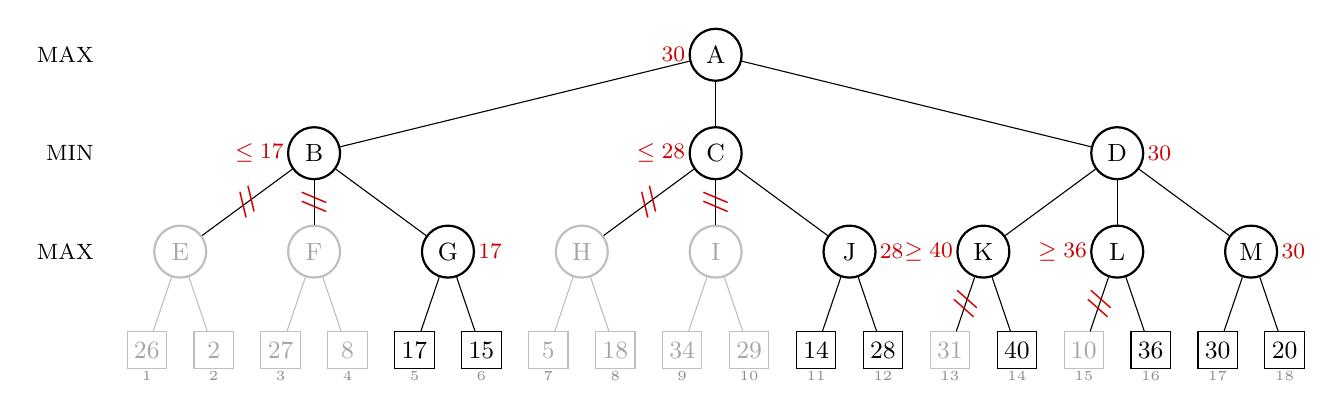
\begin{tikzpicture}[scale=1.0, every node/.style={transform shape}, gc/.style={draw, thick, circle, minimum size=6.6mm, inner sep=0pt, font=\small}, gl/.style={draw, rectangle, minimum width=5mm, minimum height=4.6mm, inner sep=1pt, font=\small}, gx/.style={draw=black!25, text=black!35}, val/.style={font=\footnotesize\bfseries, text=red!80!black, inner sep=1pt}]
\node[font=\footnotesize, anchor=east] at (-0.55,0.00) {MAX};
\node[font=\footnotesize, anchor=east] at (-0.55,-1.25) {MIN};
\node[font=\footnotesize, anchor=east] at (-0.55,-2.50) {MAX};
\node[gc, label={[val]left:$30$}] (n30) at (7.225,0.000) {A};
\node[gc, label={[val]left:$\le17$}] (n9) at (2.125,-1.250) {B};
\node[gc, gx] (n2) at (0.425,-2.500) {E};
\node[gl, gx, label={[font=\tiny, text=black!45, inner sep=1pt]below:1}] (n0) at (0.000,-3.750) {26};
\node[gl, gx, label={[font=\tiny, text=black!45, inner sep=1pt]below:2}] (n1) at (0.850,-3.750) {2};
\node[gc, gx] (n5) at (2.125,-2.500) {F};
\node[gl, gx, label={[font=\tiny, text=black!45, inner sep=1pt]below:3}] (n3) at (1.700,-3.750) {27};
\node[gl, gx, label={[font=\tiny, text=black!45, inner sep=1pt]below:4}] (n4) at (2.550,-3.750) {8};
\node[gc, label={[val]right:$17$}] (n8) at (3.825,-2.500) {G};
\node[gl, label={[font=\tiny, text=black!45, inner sep=1pt]below:5}] (n6) at (3.400,-3.750) {17};
\node[gl, label={[font=\tiny, text=black!45, inner sep=1pt]below:6}] (n7) at (4.250,-3.750) {15};
\node[gc, label={[val]left:$\le28$}] (n19) at (7.225,-1.250) {C};
\node[gc, gx] (n12) at (5.525,-2.500) {H};
\node[gl, gx, label={[font=\tiny, text=black!45, inner sep=1pt]below:7}] (n10) at (5.100,-3.750) {5};
\node[gl, gx, label={[font=\tiny, text=black!45, inner sep=1pt]below:8}] (n11) at (5.950,-3.750) {18};
\node[gc, gx] (n15) at (7.225,-2.500) {I};
\node[gl, gx, label={[font=\tiny, text=black!45, inner sep=1pt]below:9}] (n13) at (6.800,-3.750) {34};
\node[gl, gx, label={[font=\tiny, text=black!45, inner sep=1pt]below:10}] (n14) at (7.650,-3.750) {29};
\node[gc, label={[val]right:$28$}] (n18) at (8.925,-2.500) {J};
\node[gl, label={[font=\tiny, text=black!45, inner sep=1pt]below:11}] (n16) at (8.500,-3.750) {14};
\node[gl, label={[font=\tiny, text=black!45, inner sep=1pt]below:12}] (n17) at (9.350,-3.750) {28};
\node[gc, label={[val]right:$30$}] (n29) at (12.325,-1.250) {D};
\node[gc, label={[val]left:$\ge40$}] (n22) at (10.625,-2.500) {K};
\node[gl, gx, label={[font=\tiny, text=black!45, inner sep=1pt]below:13}] (n20) at (10.200,-3.750) {31};
\node[gl, label={[font=\tiny, text=black!45, inner sep=1pt]below:14}] (n21) at (11.050,-3.750) {40};
\node[gc, label={[val]left:$\ge36$}] (n25) at (12.325,-2.500) {L};
\node[gl, gx, label={[font=\tiny, text=black!45, inner sep=1pt]below:15}] (n23) at (11.900,-3.750) {10};
\node[gl, label={[font=\tiny, text=black!45, inner sep=1pt]below:16}] (n24) at (12.750,-3.750) {36};
\node[gc, label={[val]right:$30$}] (n28) at (14.025,-2.500) {M};
\node[gl, label={[font=\tiny, text=black!45, inner sep=1pt]below:17}] (n26) at (13.600,-3.750) {30};
\node[gl, label={[font=\tiny, text=black!45, inner sep=1pt]below:18}] (n27) at (14.450,-3.750) {20};
\draw (n30) -- (n9);
\draw (n30) -- (n19);
\draw (n30) -- (n29);
\draw (n9) -- (n2) node[midway, sloped, text=red!80!black, font=\small\bfseries, inner sep=0pt]{/\!/};
\draw (n9) -- (n5) node[midway, sloped, text=red!80!black, font=\small\bfseries, inner sep=0pt]{/\!/};
\draw (n9) -- (n8);
\draw[black!25] (n2) -- (n0);
\draw[black!25] (n2) -- (n1);
\draw[black!25] (n5) -- (n3);
\draw[black!25] (n5) -- (n4);
\draw (n8) -- (n6);
\draw (n8) -- (n7);
\draw (n19) -- (n12) node[midway, sloped, text=red!80!black, font=\small\bfseries, inner sep=0pt]{/\!/};
\draw (n19) -- (n15) node[midway, sloped, text=red!80!black, font=\small\bfseries, inner sep=0pt]{/\!/};
\draw (n19) -- (n18);
\draw[black!25] (n12) -- (n10);
\draw[black!25] (n12) -- (n11);
\draw[black!25] (n15) -- (n13);
\draw[black!25] (n15) -- (n14);
\draw (n18) -- (n16);
\draw (n18) -- (n17);
\draw (n29) -- (n22);
\draw (n29) -- (n25);
\draw (n29) -- (n28);
\draw (n22) -- (n20) node[midway, sloped, text=red!80!black, font=\small\bfseries, inner sep=0pt]{/\!/};
\draw (n22) -- (n21);
\draw (n25) -- (n23) node[midway, sloped, text=red!80!black, font=\small\bfseries, inner sep=0pt]{/\!/};
\draw (n25) -- (n24);
\draw (n28) -- (n26);
\draw (n28) -- (n27);
\end{tikzpicture}
\end{adjustbox}
\end{center}\begin{itemize}[leftmargin=1.5em,itemsep=1pt]
\item At MAX node \textbf{L}, after leaf \#16: $v=36 \ge \beta=30$ $\Rightarrow$ prune leaf \#15. (MIN at D already has an alternative worth $\beta=30$, so it will never let play reach L.)
\item At MAX node \textbf{K}, after leaf \#14: $v=40 \ge \beta=30$ $\Rightarrow$ prune leaf \#13. (MIN at D already has an alternative worth $\beta=30$, so it will never let play reach K.)
\item At MIN node \textbf{C}, after child J: $v=28 \le \alpha=30$ $\Rightarrow$ prune I (leaves \#9--\#10), H (leaves \#7--\#8). (MAX at A already has an alternative worth $\alpha=30$, so it will never let play reach C.)
\item At MIN node \textbf{B}, after child G: $v=17 \le \alpha=30$ $\Rightarrow$ prune F (leaves \#3--\#4), E (leaves \#1--\#2). (MAX at A already has an alternative worth $\alpha=30$, so it will never let play reach B.)
\end{itemize}Pruned leaves: \#1, \#2, \#3, \#4, \#7, \#8, \#9, \#10, \#13, \#15 (10) instead of 2. Going right to left, MAX first explores D, the best child (value 30), so $\alpha$ is high at once and the other MIN nodes are cut as soon as a child is $\le\alpha$: good move ordering is what makes alpha-beta efficient.
\end{solbox}
\question{5}Consider the game tree below, in which \textbf{MIN moves first}.\begin{center}
\begin{adjustbox}{max width=\linewidth}
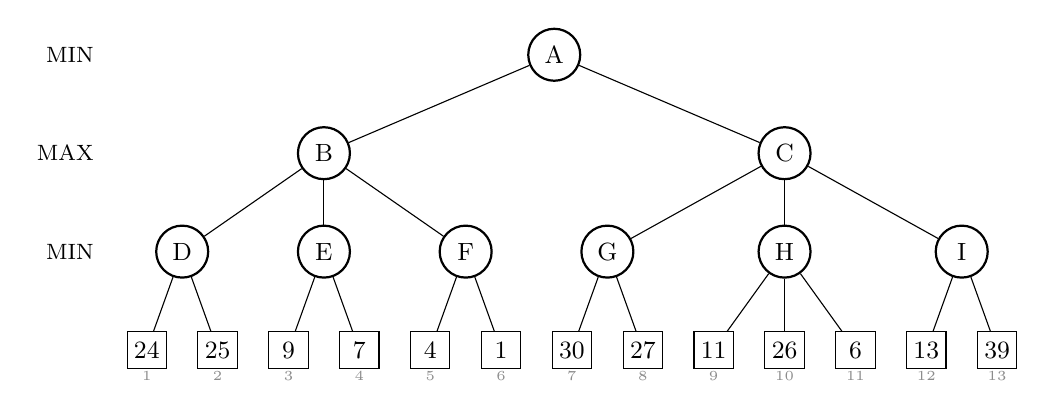
\begin{tikzpicture}[scale=1.0, every node/.style={transform shape}, gc/.style={draw, thick, circle, minimum size=6.6mm, inner sep=0pt, font=\small}, gl/.style={draw, rectangle, minimum width=5mm, minimum height=4.6mm, inner sep=1pt, font=\small}, gx/.style={draw=black!25, text=black!35}, val/.style={font=\footnotesize\bfseries, text=red!80!black, inner sep=1pt}]
\node[font=\footnotesize, anchor=east] at (-0.55,0.00) {MIN};
\node[font=\footnotesize, anchor=east] at (-0.55,-1.25) {MAX};
\node[font=\footnotesize, anchor=east] at (-0.55,-2.50) {MIN};
\node[gc] (n21) at (5.175,0.000) {A};
\node[gc] (n9) at (2.250,-1.250) {B};
\node[gc] (n2) at (0.450,-2.500) {D};
\node[gl, label={[font=\tiny, text=black!45, inner sep=1pt]below:1}] (n0) at (0.000,-3.750) {24};
\node[gl, label={[font=\tiny, text=black!45, inner sep=1pt]below:2}] (n1) at (0.900,-3.750) {25};
\node[gc] (n5) at (2.250,-2.500) {E};
\node[gl, label={[font=\tiny, text=black!45, inner sep=1pt]below:3}] (n3) at (1.800,-3.750) {9};
\node[gl, label={[font=\tiny, text=black!45, inner sep=1pt]below:4}] (n4) at (2.700,-3.750) {7};
\node[gc] (n8) at (4.050,-2.500) {F};
\node[gl, label={[font=\tiny, text=black!45, inner sep=1pt]below:5}] (n6) at (3.600,-3.750) {4};
\node[gl, label={[font=\tiny, text=black!45, inner sep=1pt]below:6}] (n7) at (4.500,-3.750) {1};
\node[gc] (n20) at (8.100,-1.250) {C};
\node[gc] (n12) at (5.850,-2.500) {G};
\node[gl, label={[font=\tiny, text=black!45, inner sep=1pt]below:7}] (n10) at (5.400,-3.750) {30};
\node[gl, label={[font=\tiny, text=black!45, inner sep=1pt]below:8}] (n11) at (6.300,-3.750) {27};
\node[gc] (n16) at (8.100,-2.500) {H};
\node[gl, label={[font=\tiny, text=black!45, inner sep=1pt]below:9}] (n13) at (7.200,-3.750) {11};
\node[gl, label={[font=\tiny, text=black!45, inner sep=1pt]below:10}] (n14) at (8.100,-3.750) {26};
\node[gl, label={[font=\tiny, text=black!45, inner sep=1pt]below:11}] (n15) at (9.000,-3.750) {6};
\node[gc] (n19) at (10.350,-2.500) {I};
\node[gl, label={[font=\tiny, text=black!45, inner sep=1pt]below:12}] (n17) at (9.900,-3.750) {13};
\node[gl, label={[font=\tiny, text=black!45, inner sep=1pt]below:13}] (n18) at (10.800,-3.750) {39};
\draw (n21) -- (n9);
\draw (n21) -- (n20);
\draw (n9) -- (n2);
\draw (n9) -- (n5);
\draw (n9) -- (n8);
\draw (n2) -- (n0);
\draw (n2) -- (n1);
\draw (n5) -- (n3);
\draw (n5) -- (n4);
\draw (n8) -- (n6);
\draw (n8) -- (n7);
\draw (n20) -- (n12);
\draw (n20) -- (n16);
\draw (n20) -- (n19);
\draw (n12) -- (n10);
\draw (n12) -- (n11);
\draw (n16) -- (n13);
\draw (n16) -- (n14);
\draw (n16) -- (n15);
\draw (n19) -- (n17);
\draw (n19) -- (n18);
\end{tikzpicture}
\end{adjustbox}
\end{center}
\subq{(a)}Note the minimax value of every node (no pruning).
\begin{solbox}
\begin{center}\small \begin{tabular}{|l|c|c|c|c|c|c|c|c|c|}\hline
\textbf{Node} & \textbf{A} & \textbf{B} & \textbf{C} & \textbf{D} & \textbf{E} & \textbf{F} & \textbf{G} & \textbf{H} & \textbf{I}\\ \hline
Minimax & \textcolor{blue!60!black}{24} & \textcolor{blue!60!black}{24} & \textcolor{blue!60!black}{27} & \textcolor{blue!60!black}{24} & \textcolor{blue!60!black}{7} & \textcolor{blue!60!black}{1} & \textcolor{blue!60!black}{27} & \textcolor{blue!60!black}{6} & \textcolor{blue!60!black}{13}\\[1.5mm] \hline
\end{tabular}\end{center}Root value $=24$; MIN moves to \textbf{B}.
\end{solbox}
\subq{(b)}Show where alpha-beta pruning occurs (left to right) by crossing out the corresponding branches, and briefly explain each case.
\begin{solbox}
\begin{center}
\begin{adjustbox}{max width=\linewidth}
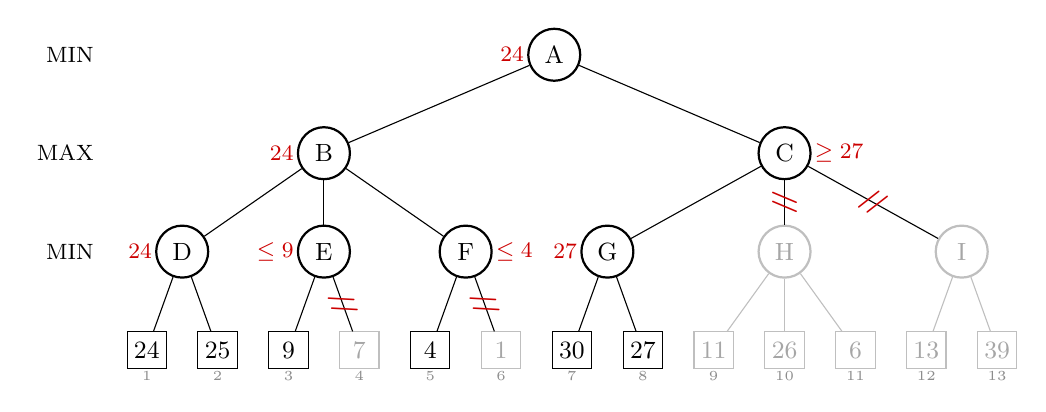
\begin{tikzpicture}[scale=1.0, every node/.style={transform shape}, gc/.style={draw, thick, circle, minimum size=6.6mm, inner sep=0pt, font=\small}, gl/.style={draw, rectangle, minimum width=5mm, minimum height=4.6mm, inner sep=1pt, font=\small}, gx/.style={draw=black!25, text=black!35}, val/.style={font=\footnotesize\bfseries, text=red!80!black, inner sep=1pt}]
\node[font=\footnotesize, anchor=east] at (-0.55,0.00) {MIN};
\node[font=\footnotesize, anchor=east] at (-0.55,-1.25) {MAX};
\node[font=\footnotesize, anchor=east] at (-0.55,-2.50) {MIN};
\node[gc, label={[val]left:$24$}] (n21) at (5.175,0.000) {A};
\node[gc, label={[val]left:$24$}] (n9) at (2.250,-1.250) {B};
\node[gc, label={[val]left:$24$}] (n2) at (0.450,-2.500) {D};
\node[gl, label={[font=\tiny, text=black!45, inner sep=1pt]below:1}] (n0) at (0.000,-3.750) {24};
\node[gl, label={[font=\tiny, text=black!45, inner sep=1pt]below:2}] (n1) at (0.900,-3.750) {25};
\node[gc, label={[val]left:$\le9$}] (n5) at (2.250,-2.500) {E};
\node[gl, label={[font=\tiny, text=black!45, inner sep=1pt]below:3}] (n3) at (1.800,-3.750) {9};
\node[gl, gx, label={[font=\tiny, text=black!45, inner sep=1pt]below:4}] (n4) at (2.700,-3.750) {7};
\node[gc, label={[val]right:$\le4$}] (n8) at (4.050,-2.500) {F};
\node[gl, label={[font=\tiny, text=black!45, inner sep=1pt]below:5}] (n6) at (3.600,-3.750) {4};
\node[gl, gx, label={[font=\tiny, text=black!45, inner sep=1pt]below:6}] (n7) at (4.500,-3.750) {1};
\node[gc, label={[val]right:$\ge27$}] (n20) at (8.100,-1.250) {C};
\node[gc, label={[val]left:$27$}] (n12) at (5.850,-2.500) {G};
\node[gl, label={[font=\tiny, text=black!45, inner sep=1pt]below:7}] (n10) at (5.400,-3.750) {30};
\node[gl, label={[font=\tiny, text=black!45, inner sep=1pt]below:8}] (n11) at (6.300,-3.750) {27};
\node[gc, gx] (n16) at (8.100,-2.500) {H};
\node[gl, gx, label={[font=\tiny, text=black!45, inner sep=1pt]below:9}] (n13) at (7.200,-3.750) {11};
\node[gl, gx, label={[font=\tiny, text=black!45, inner sep=1pt]below:10}] (n14) at (8.100,-3.750) {26};
\node[gl, gx, label={[font=\tiny, text=black!45, inner sep=1pt]below:11}] (n15) at (9.000,-3.750) {6};
\node[gc, gx] (n19) at (10.350,-2.500) {I};
\node[gl, gx, label={[font=\tiny, text=black!45, inner sep=1pt]below:12}] (n17) at (9.900,-3.750) {13};
\node[gl, gx, label={[font=\tiny, text=black!45, inner sep=1pt]below:13}] (n18) at (10.800,-3.750) {39};
\draw (n21) -- (n9);
\draw (n21) -- (n20);
\draw (n9) -- (n2);
\draw (n9) -- (n5);
\draw (n9) -- (n8);
\draw (n2) -- (n0);
\draw (n2) -- (n1);
\draw (n5) -- (n3);
\draw (n5) -- (n4) node[midway, sloped, text=red!80!black, font=\small\bfseries, inner sep=0pt]{/\!/};
\draw (n8) -- (n6);
\draw (n8) -- (n7) node[midway, sloped, text=red!80!black, font=\small\bfseries, inner sep=0pt]{/\!/};
\draw (n20) -- (n12);
\draw (n20) -- (n16) node[midway, sloped, text=red!80!black, font=\small\bfseries, inner sep=0pt]{/\!/};
\draw (n20) -- (n19) node[midway, sloped, text=red!80!black, font=\small\bfseries, inner sep=0pt]{/\!/};
\draw (n12) -- (n10);
\draw (n12) -- (n11);
\draw[black!25] (n16) -- (n13);
\draw[black!25] (n16) -- (n14);
\draw[black!25] (n16) -- (n15);
\draw[black!25] (n19) -- (n17);
\draw[black!25] (n19) -- (n18);
\end{tikzpicture}
\end{adjustbox}
\end{center}\begin{center}\small\begin{tabular}{c c c c c}\toprule Node & Type & On entry & When it returns & Value returned\\\midrule A & MIN & $\alpha=-\infty,\ \beta=+\infty$ & $\alpha=-\infty,\ \beta=24$ & $24$ \\
B & MAX & $\alpha=-\infty,\ \beta=+\infty$ & $\alpha=24,\ \beta=+\infty$ & $24$ \\
D & MIN & $\alpha=-\infty,\ \beta=+\infty$ & $\alpha=-\infty,\ \beta=24$ & $24$ \\
E & MIN & $\alpha=24,\ \beta=+\infty$ & $\alpha=24,\ \beta=9$ & $\le 9$ \\
F & MIN & $\alpha=24,\ \beta=+\infty$ & $\alpha=24,\ \beta=4$ & $\le 4$ \\
C & MAX & $\alpha=-\infty,\ \beta=24$ & $\alpha=27,\ \beta=24$ & $\ge 27$ \\
G & MIN & $\alpha=-\infty,\ \beta=24$ & $\alpha=-\infty,\ \beta=24$ & $27$ \\\bottomrule\end{tabular}\end{center}\begin{itemize}[leftmargin=1.5em,itemsep=1pt]
\item At MIN node \textbf{E}, after leaf \#3: $v=9 \le \alpha=24$ $\Rightarrow$ prune leaf \#4. (MAX at B already has an alternative worth $\alpha=24$, so it will never let play reach E.)
\item At MIN node \textbf{F}, after leaf \#5: $v=4 \le \alpha=24$ $\Rightarrow$ prune leaf \#6. (MAX at B already has an alternative worth $\alpha=24$, so it will never let play reach F.)
\item At MAX node \textbf{C}, after child G: $v=27 \ge \beta=24$ $\Rightarrow$ prune H (leaves \#9--\#11), I (leaves \#12--\#13). (MIN at A already has an alternative worth $\beta=24$, so it will never let play reach C.)
\end{itemize}Leaves evaluated: 6 of 13; never evaluated: \#4, \#6, \#9, \#10, \#11, \#12, \#13.
\end{solbox}
\question{6}Three players A, B, C move in turn. Each leaf gives the utility vector $(u_A,u_B,u_C)$ and every player maximises its own component.\begin{center}
\begin{adjustbox}{max width=\linewidth}
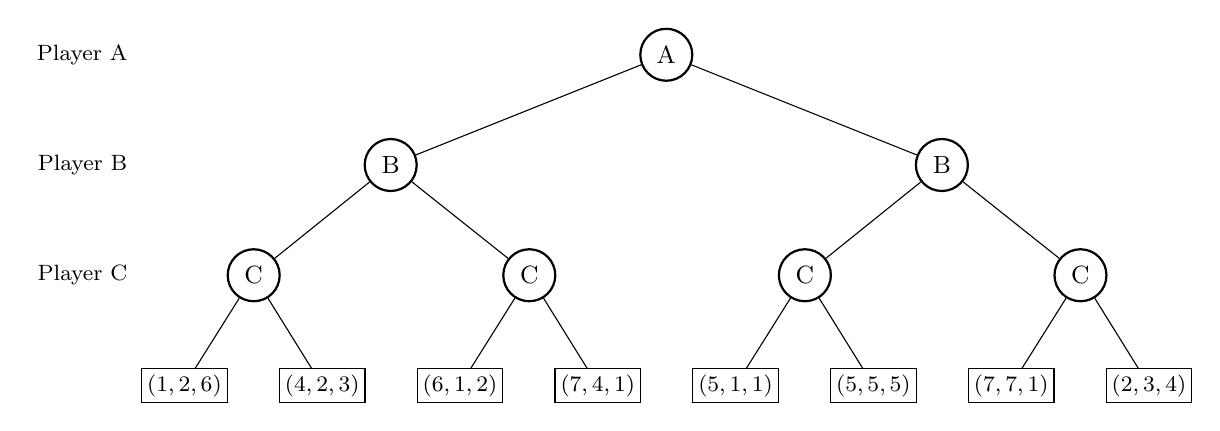
\begin{tikzpicture}[pn/.style={draw, thick, circle, minimum size=6.6mm, inner sep=0pt, font=\small}, lv/.style={draw, rectangle, inner sep=2pt, font=\footnotesize}]
\node[font=\footnotesize, anchor=east] at (-0.6,0.00) {Player A};
\node[font=\footnotesize, anchor=east] at (-0.6,-1.40) {Player B};
\node[font=\footnotesize, anchor=east] at (-0.6,-2.80) {Player C};
\node[pn] (p) at (6.12,0.00) {A};
\node[pn] (p0) at (2.62,-1.40) {B};
\node[pn] (p00) at (0.88,-2.80) {C};
\node[lv] (p000) at (0.00,-4.20) {$(1,2,6)$};
\draw (p00) -- (p000);
\node[lv] (p001) at (1.75,-4.20) {$(4,2,3)$};
\draw (p00) -- (p001);
\draw (p0) -- (p00);
\node[pn] (p01) at (4.38,-2.80) {C};
\node[lv] (p010) at (3.50,-4.20) {$(6,1,2)$};
\draw (p01) -- (p010);
\node[lv] (p011) at (5.25,-4.20) {$(7,4,1)$};
\draw (p01) -- (p011);
\draw (p0) -- (p01);
\draw (p) -- (p0);
\node[pn] (p1) at (9.62,-1.40) {B};
\node[pn] (p10) at (7.88,-2.80) {C};
\node[lv] (p100) at (7.00,-4.20) {$(5,1,1)$};
\draw (p10) -- (p100);
\node[lv] (p101) at (8.75,-4.20) {$(5,5,5)$};
\draw (p10) -- (p101);
\draw (p1) -- (p10);
\node[pn] (p11) at (11.38,-2.80) {C};
\node[lv] (p110) at (10.50,-4.20) {$(7,7,1)$};
\draw (p11) -- (p110);
\node[lv] (p111) at (12.25,-4.20) {$(2,3,4)$};
\draw (p11) -- (p111);
\draw (p1) -- (p11);
\draw (p) -- (p1);
\end{tikzpicture}
\end{adjustbox}
\end{center}
\subq{(a)}Back up the utility vectors to every node. Which move does A make?
\begin{solbox}
\begin{center}
\begin{adjustbox}{max width=\linewidth}
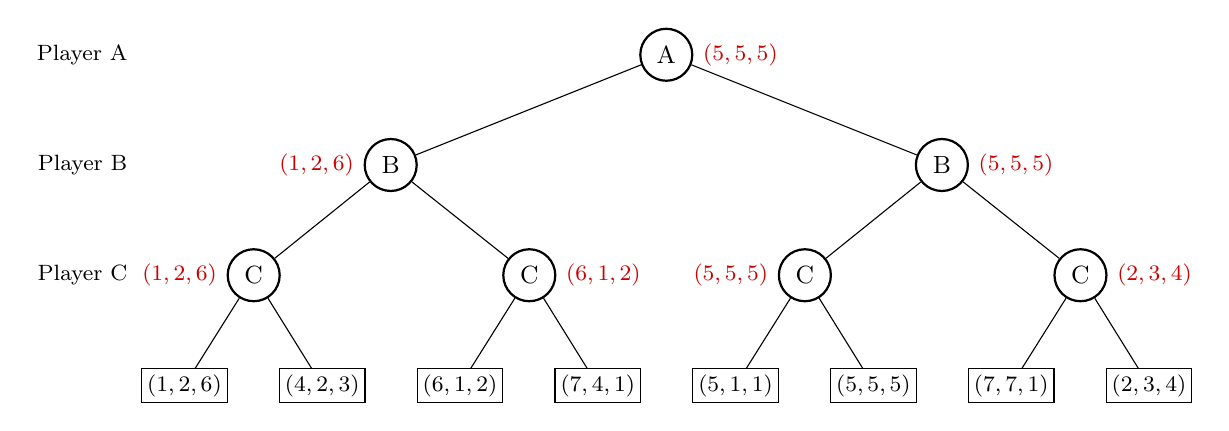
\begin{tikzpicture}[pn/.style={draw, thick, circle, minimum size=6.6mm, inner sep=0pt, font=\small}, lv/.style={draw, rectangle, inner sep=2pt, font=\footnotesize}]
\node[font=\footnotesize, anchor=east] at (-0.6,0.00) {Player A};
\node[font=\footnotesize, anchor=east] at (-0.6,-1.40) {Player B};
\node[font=\footnotesize, anchor=east] at (-0.6,-2.80) {Player C};
\node[pn, label={[font=\footnotesize\bfseries, text=red!80!black]right:$(5,5,5)$}] (p) at (6.12,0.00) {A};
\node[pn, label={[font=\footnotesize\bfseries, text=red!80!black]left:$(1,2,6)$}] (p0) at (2.62,-1.40) {B};
\node[pn, label={[font=\footnotesize\bfseries, text=red!80!black]left:$(1,2,6)$}] (p00) at (0.88,-2.80) {C};
\node[lv] (p000) at (0.00,-4.20) {$(1,2,6)$};
\draw (p00) -- (p000);
\node[lv] (p001) at (1.75,-4.20) {$(4,2,3)$};
\draw (p00) -- (p001);
\draw (p0) -- (p00);
\node[pn, label={[font=\footnotesize\bfseries, text=red!80!black]right:$(6,1,2)$}] (p01) at (4.38,-2.80) {C};
\node[lv] (p010) at (3.50,-4.20) {$(6,1,2)$};
\draw (p01) -- (p010);
\node[lv] (p011) at (5.25,-4.20) {$(7,4,1)$};
\draw (p01) -- (p011);
\draw (p0) -- (p01);
\draw (p) -- (p0);
\node[pn, label={[font=\footnotesize\bfseries, text=red!80!black]right:$(5,5,5)$}] (p1) at (9.62,-1.40) {B};
\node[pn, label={[font=\footnotesize\bfseries, text=red!80!black]left:$(5,5,5)$}] (p10) at (7.88,-2.80) {C};
\node[lv] (p100) at (7.00,-4.20) {$(5,1,1)$};
\draw (p10) -- (p100);
\node[lv] (p101) at (8.75,-4.20) {$(5,5,5)$};
\draw (p10) -- (p101);
\draw (p1) -- (p10);
\node[pn, label={[font=\footnotesize\bfseries, text=red!80!black]right:$(2,3,4)$}] (p11) at (11.38,-2.80) {C};
\node[lv] (p110) at (10.50,-4.20) {$(7,7,1)$};
\draw (p11) -- (p110);
\node[lv] (p111) at (12.25,-4.20) {$(2,3,4)$};
\draw (p11) -- (p111);
\draw (p1) -- (p11);
\draw (p) -- (p1);
\end{tikzpicture}
\end{adjustbox}
\end{center}Root $=(5,5,5)$: A moves to the right subtree (A gets 5 instead of 1).
\end{solbox}
\subq{(b)}The game is not zero-sum. Explain, using this tree, why alliances may form and why they may be broken.
\begin{solbox}
$(5,5,5)$ is good for everybody, so A and B both prefer the right subtree: collaboration can arise. But each player keeps an alliance only while it serves its own utility: at the right-most C node, C prefers $(2,3,4)$ to $(7,7,1)$, which A and B would both like.
\end{solbox}
\question{7}Consider the MCTS tree below; rewards are scores in $[0,10]$ for the root player. Use $\mathrm{UCB1}=\bar V_i+C\sqrt{\ln N/n_i}$ with $C=2$ (unvisited $=\infty$, ties to the left; a never-visited leaf is rolled out directly, otherwise all its children are added and the rollout starts at the first). Expansion: $A\to A_1,A_2,A_3$; $B\to B_1,B_2,B_3$; $X_i\to X_{i1},X_{i2}$; $X_{ij}\to X_{ij1},X_{ij2}$.\begin{center}
\begin{adjustbox}{max width=\linewidth}
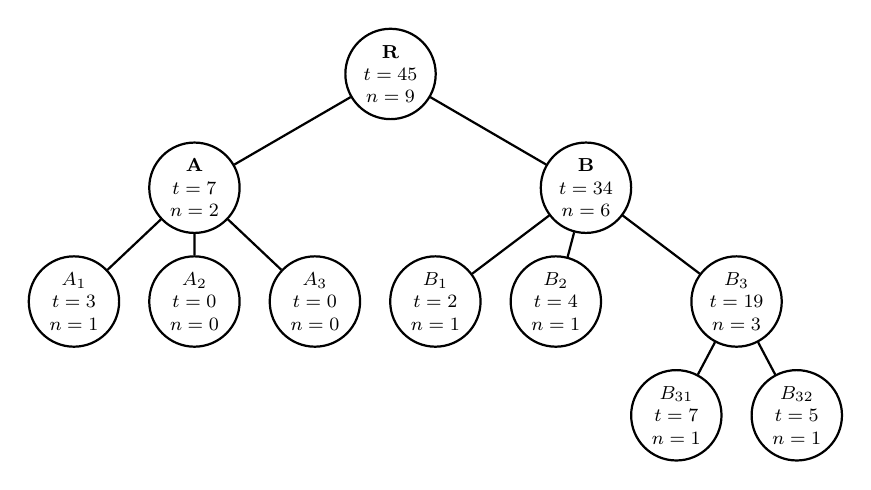
\begin{tikzpicture}[scale=0.85, every node/.style={transform shape}, mn/.style={draw, thick, circle, align=center, font=\footnotesize, inner sep=0.5pt, minimum size=13.5mm}]
\node[mn] (m1) at (4.73,0.00) {\textbf{R}\\ $t=45$\\ $n=9$};
\node[mn] (m2) at (1.80,-1.70) {\textbf{A}\\ $t=7$\\ $n=2$};
\node[mn] (m3) at (0.00,-3.40) {\textbf{$A_{1}$}\\ $t=3$\\ $n=1$};
\draw[thick] (m2) -- (m3);
\node[mn] (m4) at (1.80,-3.40) {\textbf{$A_{2}$}\\ $t=0$\\ $n=0$};
\draw[thick] (m2) -- (m4);
\node[mn] (m5) at (3.60,-3.40) {\textbf{$A_{3}$}\\ $t=0$\\ $n=0$};
\draw[thick] (m2) -- (m5);
\draw[thick] (m1) -- (m2);
\node[mn] (m6) at (7.65,-1.70) {\textbf{B}\\ $t=34$\\ $n=6$};
\node[mn] (m7) at (5.40,-3.40) {\textbf{$B_{1}$}\\ $t=2$\\ $n=1$};
\draw[thick] (m6) -- (m7);
\node[mn] (m8) at (7.20,-3.40) {\textbf{$B_{2}$}\\ $t=4$\\ $n=1$};
\draw[thick] (m6) -- (m8);
\node[mn] (m9) at (9.90,-3.40) {\textbf{$B_{3}$}\\ $t=19$\\ $n=3$};
\node[mn] (m10) at (9.00,-5.10) {\textbf{$B_{31}$}\\ $t=7$\\ $n=1$};
\draw[thick] (m9) -- (m10);
\node[mn] (m11) at (10.80,-5.10) {\textbf{$B_{32}$}\\ $t=5$\\ $n=1$};
\draw[thick] (m9) -- (m11);
\draw[thick] (m6) -- (m9);
\draw[thick] (m1) -- (m6);
\end{tikzpicture}
\end{adjustbox}
\end{center}
\subq{(a)}Perform three iterations whose rollouts return $0,\ 1,\ 10$ (in order). Give the UCB1 values at every selection step and draw the final tree.
\begin{solbox}
\textbf{Iteration 1.}
\begin{itemize}[leftmargin=1.5em,itemsep=1pt]
\item \emph{Selection} at R ($N=9$): A: $\frac{7}{2} + 2\sqrt{\frac{\ln 9}{2}} = 5.596$; B: $\frac{34}{6} + 2\sqrt{\frac{\ln 9}{6}} = 6.877$ $\Rightarrow$ go to \textbf{B}.
\item \emph{Selection} at B ($N=6$): $B_{1}$: $\frac{2}{1} + 2\sqrt{\frac{\ln 6}{1}} = 4.677$; $B_{2}$: $\frac{4}{1} + 2\sqrt{\frac{\ln 6}{1}} = 6.677$; $B_{3}$: $\frac{19}{3} + 2\sqrt{\frac{\ln 6}{3}} = 7.879$ $\Rightarrow$ go to \textbf{$B_{3}$}.
\item \emph{Selection} at $B_{3}$ ($N=3$): $B_{31}$: $\frac{7}{1} + 2\sqrt{\frac{\ln 3}{1}} = 9.096$; $B_{32}$: $\frac{5}{1} + 2\sqrt{\frac{\ln 3}{1}} = 7.096$ $\Rightarrow$ go to \textbf{$B_{31}$}.
\item \emph{Expansion}: $B_{31}$ was visited before ($n>0$) and has no children $\Rightarrow$ add $B_{311}$, $B_{312}$; roll out from the first one, \textbf{$B_{311}$}.
\item \emph{Simulation}: rollout from $B_{311}$ returns $0$.
\item \emph{Backpropagation}: add $0$ to $t$ and $1$ to $n$ for R $\to$ B $\to$ $B_{3}$ $\to$ $B_{31}$ $\to$ $B_{311}$.
\end{itemize}
\textit{Statistics ($t/n$) after iteration 1:} R: 45/10, A: 7/2, $A_{1}$: 3/1, $A_{2}$: 0/0, $A_{3}$: 0/0, B: 34/7, $B_{1}$: 2/1, $B_{2}$: 4/1, $B_{3}$: 19/4, $B_{31}$: 7/2, $B_{311}$: 0/1, $B_{312}$: 0/0, $B_{32}$: 5/1.

\smallskip
\textbf{Iteration 2.}
\begin{itemize}[leftmargin=1.5em,itemsep=1pt]
\item \emph{Selection} at R ($N=10$): A: $\frac{7}{2} + 2\sqrt{\frac{\ln 10}{2}} = 5.646$; B: $\frac{34}{7} + 2\sqrt{\frac{\ln 10}{7}} = 6.004$ $\Rightarrow$ go to \textbf{B}.
\item \emph{Selection} at B ($N=7$): $B_{1}$: $\frac{2}{1} + 2\sqrt{\frac{\ln 7}{1}} = 4.790$; $B_{2}$: $\frac{4}{1} + 2\sqrt{\frac{\ln 7}{1}} = 6.790$; $B_{3}$: $\frac{19}{4} + 2\sqrt{\frac{\ln 7}{4}} = 6.145$ $\Rightarrow$ go to \textbf{$B_{2}$}.
\item \emph{Expansion}: $B_{2}$ was visited before ($n>0$) and has no children $\Rightarrow$ add $B_{21}$, $B_{22}$; roll out from the first one, \textbf{$B_{21}$}.
\item \emph{Simulation}: rollout from $B_{21}$ returns $1$.
\item \emph{Backpropagation}: add $1$ to $t$ and $1$ to $n$ for R $\to$ B $\to$ $B_{2}$ $\to$ $B_{21}$.
\end{itemize}
\textit{Statistics ($t/n$) after iteration 2:} R: 46/11, A: 7/2, $A_{1}$: 3/1, $A_{2}$: 0/0, $A_{3}$: 0/0, B: 35/8, $B_{1}$: 2/1, $B_{2}$: 5/2, $B_{21}$: 1/1, $B_{22}$: 0/0, $B_{3}$: 19/4, $B_{31}$: 7/2, $B_{311}$: 0/1, $B_{312}$: 0/0, $B_{32}$: 5/1.

\smallskip
\textbf{Iteration 3.}
\begin{itemize}[leftmargin=1.5em,itemsep=1pt]
\item \emph{Selection} at R ($N=11$): A: $\frac{7}{2} + 2\sqrt{\frac{\ln 11}{2}} = 5.690$; B: $\frac{35}{8} + 2\sqrt{\frac{\ln 11}{8}} = 5.470$ $\Rightarrow$ go to \textbf{A}.
\item \emph{Selection} at A ($N=2$): $A_{1}$: $\frac{3}{1} + 2\sqrt{\frac{\ln 2}{1}} = 4.665$; $A_{2}$: $\infty$ (unvisited); $A_{3}$: $\infty$ (unvisited) $\Rightarrow$ go to \textbf{$A_{2}$}.
\item \emph{Expansion}: none --- \textbf{$A_{2}$} has $n=0$, so we roll out directly from it.
\item \emph{Simulation}: rollout from $A_{2}$ returns $10$.
\item \emph{Backpropagation}: add $10$ to $t$ and $1$ to $n$ for R $\to$ A $\to$ $A_{2}$.
\end{itemize}
\textit{Statistics ($t/n$) after iteration 3:} R: 56/12, A: 17/3, $A_{1}$: 3/1, $A_{2}$: 10/1, $A_{3}$: 0/0, B: 35/8, $B_{1}$: 2/1, $B_{2}$: 5/2, $B_{21}$: 1/1, $B_{22}$: 0/0, $B_{3}$: 19/4, $B_{31}$: 7/2, $B_{311}$: 0/1, $B_{312}$: 0/0, $B_{32}$: 5/1.\par Final tree:\begin{center}
\begin{adjustbox}{max width=\linewidth}
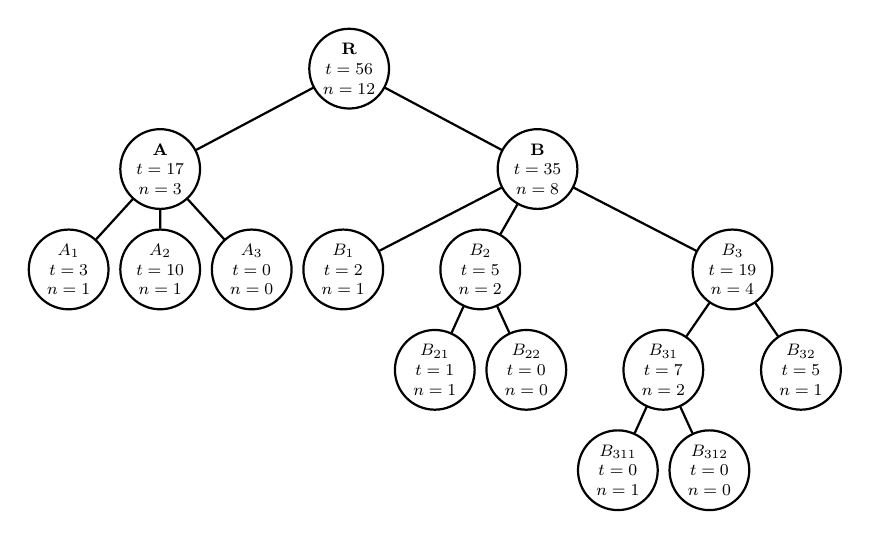
\begin{tikzpicture}[scale=0.75, every node/.style={transform shape}, mn/.style={draw, thick, circle, align=center, font=\footnotesize, inner sep=0.5pt, minimum size=13.5mm}]
\node[mn] (m1) at (4.75,0.00) {\textbf{R}\\ $t=56$\\ $n=12$};
\node[mn] (m2) at (1.55,-1.70) {\textbf{A}\\ $t=17$\\ $n=3$};
\node[mn] (m3) at (0.00,-3.40) {\textbf{$A_{1}$}\\ $t=3$\\ $n=1$};
\draw[thick] (m2) -- (m3);
\node[mn] (m4) at (1.55,-3.40) {\textbf{$A_{2}$}\\ $t=10$\\ $n=1$};
\draw[thick] (m2) -- (m4);
\node[mn] (m5) at (3.10,-3.40) {\textbf{$A_{3}$}\\ $t=0$\\ $n=0$};
\draw[thick] (m2) -- (m5);
\draw[thick] (m1) -- (m2);
\node[mn] (m6) at (7.94,-1.70) {\textbf{B}\\ $t=35$\\ $n=8$};
\node[mn] (m7) at (4.65,-3.40) {\textbf{$B_{1}$}\\ $t=2$\\ $n=1$};
\draw[thick] (m6) -- (m7);
\node[mn] (m8) at (6.97,-3.40) {\textbf{$B_{2}$}\\ $t=5$\\ $n=2$};
\node[mn] (m9) at (6.20,-5.10) {\textbf{$B_{21}$}\\ $t=1$\\ $n=1$};
\draw[thick] (m8) -- (m9);
\node[mn] (m10) at (7.75,-5.10) {\textbf{$B_{22}$}\\ $t=0$\\ $n=0$};
\draw[thick] (m8) -- (m10);
\draw[thick] (m6) -- (m8);
\node[mn] (m11) at (11.24,-3.40) {\textbf{$B_{3}$}\\ $t=19$\\ $n=4$};
\node[mn] (m12) at (10.07,-5.10) {\textbf{$B_{31}$}\\ $t=7$\\ $n=2$};
\node[mn] (m13) at (9.30,-6.80) {\textbf{$B_{311}$}\\ $t=0$\\ $n=1$};
\draw[thick] (m12) -- (m13);
\node[mn] (m14) at (10.85,-6.80) {\textbf{$B_{312}$}\\ $t=0$\\ $n=0$};
\draw[thick] (m12) -- (m14);
\draw[thick] (m11) -- (m12);
\node[mn] (m15) at (12.40,-5.10) {\textbf{$B_{32}$}\\ $t=5$\\ $n=1$};
\draw[thick] (m11) -- (m15);
\draw[thick] (m6) -- (m11);
\draw[thick] (m1) -- (m6);
\end{tikzpicture}
\end{adjustbox}
\end{center}
\end{solbox}
\subq{(b)}Which root action is chosen by the \emph{max child}, \emph{robust child} and \emph{secure child} rules (secure: maximise $\bar V_i-C\sqrt{\ln N/n_i}$, $C=2$)? What does \emph{max-robust child} recommend?
\begin{solbox}
Averages A: 5.67, B: 4.38 $\Rightarrow$ max child \textbf{A}; visits A: 3, B: 8 $\Rightarrow$ robust child \textbf{B}; lower bounds A: 3.85, B: 3.26 $\Rightarrow$ secure child \textbf{A}. Max and robust disagree, so max-robust says to keep searching until one child is best in both.
\end{solbox}
\question{8}This problem is about map colouring. Each region must be coloured Red (R), Green (G) or Blue (B), and neighbouring regions must have different colours. The constraint graph is shown below. The following questions are mutually independent.\begin{center}
\begin{adjustbox}{max width=\linewidth}
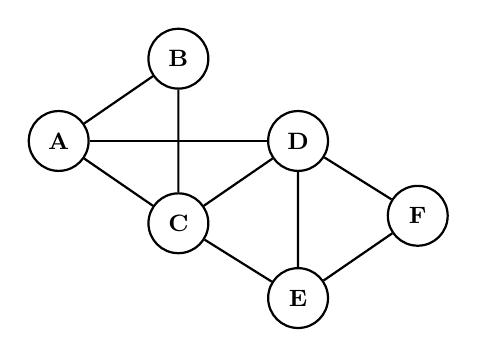
\begin{tikzpicture}[scale=0.95, every node/.style={transform shape}, cv/.style={draw, thick, circle, minimum size=8mm, inner sep=0pt, font=\small\bfseries}]
\node[cv] (A) at (0.00,1.10) {A};
\node[cv] (B) at (1.60,2.20) {B};
\node[cv] (C) at (1.60,0.00) {C};
\node[cv] (D) at (3.20,1.10) {D};
\node[cv] (E) at (3.20,-1.00) {E};
\node[cv] (F) at (4.80,0.10) {F};
\draw[thick] (A) to[] (B);
\draw[thick] (A) to[] (C);
\draw[thick] (A) to[] (D);
\draw[thick] (B) to[] (C);
\draw[thick] (C) to[] (D);
\draw[thick] (C) to[] (E);
\draw[thick] (D) to[] (E);
\draw[thick] (D) to[] (F);
\draw[thick] (E) to[] (F);
\end{tikzpicture}
\end{adjustbox}
\end{center}
\subq{(a)}\textbf{Cross out} all values that would be eliminated by \emph{forward checking} after variable B has been assigned as shown.\begin{center}\small\begin{tabular}{|l|c|c|c|c|c|c|}\hline Variables & \textbf{A} & \textbf{B} & \textbf{C} & \textbf{D} & \textbf{E} & \textbf{F}\\ \hline Domains & R\ G\ B & \textbf{R} & R\ G\ B & R\ G\ B & R\ G\ B & R\ G\ B\\ \hline\end{tabular}\end{center}
\begin{solbox}
\begin{center}\small\begin{tabular}{|l|c|c|c|c|c|c|}\hline Variables & \textbf{A} & \textbf{B} & \textbf{C} & \textbf{D} & \textbf{E} & \textbf{F}\\ \hline Domains & \textcolor{red!70!black}{\sout{R}}\ G\ B & \textbf{R}\ \textcolor{red!70!black}{\sout{G}}\ \textcolor{red!70!black}{\sout{B}} & \textcolor{red!70!black}{\sout{R}}\ G\ B & R\ G\ B & R\ G\ B & R\ G\ B\\ \hline\end{tabular}\end{center}Only the neighbours of B (A, C) lose R.
\end{solbox}
\subq{(b)}A and B have been assigned as shown, but no constraint propagation has been done yet. \textbf{Cross out} all values that would be eliminated by \emph{arc consistency} (AC-3).\begin{center}\small\begin{tabular}{|l|c|c|c|c|c|c|}\hline Variables & \textbf{A} & \textbf{B} & \textbf{C} & \textbf{D} & \textbf{E} & \textbf{F}\\ \hline Domains & \textbf{R} & \textbf{G} & R\ G\ B & R\ G\ B & R\ G\ B & R\ G\ B\\ \hline\end{tabular}\end{center}
\begin{solbox}
\begin{center}\small\begin{tabular}{|l|c|c|c|c|c|c|}\hline Variables & \textbf{A} & \textbf{B} & \textbf{C} & \textbf{D} & \textbf{E} & \textbf{F}\\ \hline Domains & \textbf{R}\ \textcolor{red!70!black}{\sout{G}}\ \textcolor{red!70!black}{\sout{B}} & \textcolor{red!70!black}{\sout{R}}\ \textbf{G}\ \textcolor{red!70!black}{\sout{B}} & \textcolor{red!70!black}{\sout{R}}\ \textcolor{red!70!black}{\sout{G}}\ B & \textcolor{red!70!black}{\sout{R}}\ G\ \textcolor{red!70!black}{\sout{B}} & R\ \textcolor{red!70!black}{\sout{G}}\ \textcolor{red!70!black}{\sout{B}} & \textcolor{red!70!black}{\sout{R}}\ \textcolor{red!70!black}{\sout{G}}\ B\\ \hline\end{tabular}\end{center}Propagation continues through the graph (unlike forward checking): every arc $X_i\to X_j$ is revised until no domain changes. Here arc consistency even leaves a single value for every variable.
\end{solbox}
\subq{(c)}Variable A is already assigned and constraint propagation has been done. \textbf{Circle} all unassigned variables that might be selected by the \emph{Minimum-Remaining-Values} (MRV) heuristic.\begin{center}\small\begin{tabular}{|l|c|c|c|c|c|c|}\hline Variables & \textbf{A} & \textbf{B} & \textbf{C} & \textbf{D} & \textbf{E} & \textbf{F}\\ \hline Domains & \textbf{R} & G\ B & G\ B & G\ B & R\ G\ B & R\ G\ B\\ \hline\end{tabular}\end{center}
\begin{solbox}
Remaining values: B: 2, C: 2, D: 2, E: 3, F: 3 $\Rightarrow$ MRV may select \textbf{B, C, D}.
\end{solbox}
\subq{(d)}Same situation. \textbf{Circle} all unassigned variables that might be selected by the \emph{Degree Heuristic}.\begin{center}\small\begin{tabular}{|l|c|c|c|c|c|c|}\hline Variables & \textbf{A} & \textbf{B} & \textbf{C} & \textbf{D} & \textbf{E} & \textbf{F}\\ \hline Domains & \textbf{R} & G\ B & G\ B & G\ B & R\ G\ B & R\ G\ B\\ \hline\end{tabular}\end{center}
\begin{solbox}
Degree = number of constraints with other \emph{unassigned} variables: B: 1, C: 3, D: 3, E: 3, F: 2 $\Rightarrow$ the degree heuristic may select \textbf{C, D, E}.
\end{solbox}
\subq{(e)}Assume no variable has been assigned yet. Solve the CSP using backtracking with \emph{forward checking}, choosing variables with MRV, then the degree heuristic (DH), and finally alphabetical order; try values in the order R, G, B. For every step give the MRV value of every region not yet coloured, and the DH values of the regions tied on the minimum MRV.
\begin{solbox}
\par \underline{Step 1}\par\begin{center}\small \begin{tabular}{|l|c|c|c|c|c|c|}\hline Variables & \textbf{A} & \textbf{B} & \textbf{C} & \textbf{D} & \textbf{E} & \textbf{F}\\ \hline MRV & \textcolor{blue!60!black}{3} & \textcolor{blue!60!black}{3} & \textcolor{blue!60!black}{3} & \textcolor{blue!60!black}{3} & \textcolor{blue!60!black}{3} & \textcolor{blue!60!black}{3}\\ \hline DH & \textcolor{blue!60!black}{3} & \textcolor{blue!60!black}{2} & \textcolor{blue!60!black}{4} & \textcolor{blue!60!black}{4} & \textcolor{blue!60!black}{3} & \textcolor{blue!60!black}{2}\\ \hline\end{tabular}\end{center}Assign to the variable \textbf{C} with the value \textbf{R} (tie on MRV and DH, broken alphabetically). Domains before this step: A=RGB, B=RGB, C=RGB, D=RGB, E=RGB, F=RGB.\par
\underline{Step 2}\par\begin{center}\small \begin{tabular}{|l|c|c|c|c|c|c|}\hline Variables & \textbf{A} & \textbf{B} & \textbf{C} & \textbf{D} & \textbf{E} & \textbf{F}\\ \hline MRV & \textcolor{blue!60!black}{2} & \textcolor{blue!60!black}{2} & -- & \textcolor{blue!60!black}{2} & \textcolor{blue!60!black}{2} & \textcolor{blue!60!black}{3}\\ \hline DH & \textcolor{blue!60!black}{2} & \textcolor{blue!60!black}{1} &  & \textcolor{blue!60!black}{3} & \textcolor{blue!60!black}{2} & \\ \hline\end{tabular}\end{center}Assign to the variable \textbf{D} with the value \textbf{G} (tie on MRV broken by DH). Domains before this step: A=GB, B=GB, C=R, D=GB, E=GB, F=RGB.\par
\underline{Step 3}\par\begin{center}\small \begin{tabular}{|l|c|c|c|c|c|c|}\hline Variables & \textbf{A} & \textbf{B} & \textbf{C} & \textbf{D} & \textbf{E} & \textbf{F}\\ \hline MRV & \textcolor{blue!60!black}{1} & \textcolor{blue!60!black}{2} & -- & -- & \textcolor{blue!60!black}{1} & \textcolor{blue!60!black}{2}\\ \hline DH & \textcolor{blue!60!black}{1} &  &  &  & \textcolor{blue!60!black}{1} & \\ \hline\end{tabular}\end{center}Assign to the variable \textbf{A} with the value \textbf{B} (tie on MRV and DH, broken alphabetically). Domains before this step: A=B, B=GB, C=R, D=G, E=B, F=RB.\par
\underline{Step 4}\par\begin{center}\small \begin{tabular}{|l|c|c|c|c|c|c|}\hline Variables & \textbf{A} & \textbf{B} & \textbf{C} & \textbf{D} & \textbf{E} & \textbf{F}\\ \hline MRV & -- & \textcolor{blue!60!black}{1} & -- & -- & \textcolor{blue!60!black}{1} & \textcolor{blue!60!black}{2}\\ \hline DH &  & \textcolor{blue!60!black}{0} &  &  & \textcolor{blue!60!black}{1} & \\ \hline\end{tabular}\end{center}Assign to the variable \textbf{E} with the value \textbf{B} (tie on MRV broken by DH). Domains before this step: A=B, B=G, C=R, D=G, E=B, F=RB.\par
\underline{Step 5}\par\begin{center}\small \begin{tabular}{|l|c|c|c|c|c|c|}\hline Variables & \textbf{A} & \textbf{B} & \textbf{C} & \textbf{D} & \textbf{E} & \textbf{F}\\ \hline MRV & -- & \textcolor{blue!60!black}{1} & -- & -- & -- & \textcolor{blue!60!black}{1}\\ \hline DH &  & \textcolor{blue!60!black}{0} &  &  &  & \textcolor{blue!60!black}{0}\\ \hline\end{tabular}\end{center}Assign to the variable \textbf{B} with the value \textbf{G} (tie on MRV and DH, broken alphabetically). Domains before this step: A=B, B=G, C=R, D=G, E=B, F=R.\par
\underline{Step 6}\par\begin{center}\small \begin{tabular}{|l|c|c|c|c|c|c|}\hline Variables & \textbf{A} & \textbf{B} & \textbf{C} & \textbf{D} & \textbf{E} & \textbf{F}\\ \hline MRV & -- & -- & -- & -- & -- & \textcolor{blue!60!black}{1}\\ \hline DH &  &  &  &  &  & \\ \hline\end{tabular}\end{center}Assign to the variable \textbf{F} with the value \textbf{R} (unique minimum MRV). Domains before this step: A=B, B=G, C=R, D=G, E=B, F=R.\par Solution: A=B, B=G, C=R, D=G, E=B, F=R. No backtracking is needed.
\end{solbox}
\question{9}4-queens as a CSP: variable $Q_i$ is the row of the queen in column $i$, with domain $\{1,2,3,4\}$.
\subq{(a)}Write the constraints.
\begin{solbox}
For all $i<j$: $Q_i\ne Q_j$ and $|Q_i-Q_j|\ne j-i$ (columns are distinct by construction).
\end{solbox}
\subq{(b)}Solve with backtracking and \emph{forward checking}, variables in the order $Q_1,\dots,Q_4$, values in increasing order. Give the domains after every assignment and draw the search tree, marking the wipe-outs.
\begin{solbox}
\begin{center}\small\begin{tabular}{c l c c c c  l}\toprule
Step & Assign & Q1 & Q2 & Q3 & Q4 & Note \\ \midrule
1 & Q1$=$1 & \textbf{1} & 34 & 24 & 23 &  \\
2 & Q2$=$3 & \textit{1} & \textbf{3} & \textcolor{red}{$\emptyset$} & 23 & \textcolor{red}{$D_{Q3}$ wiped out} \\
\multicolumn{6}{l}{\quad\textit{backtrack: undo Q2=3}} \\
3 & Q2$=$4 & \textit{1} & \textbf{4} & 2 & 3 &  \\
4 & Q3$=$2 & \textit{1} & \textit{4} & \textbf{2} & \textcolor{red}{$\emptyset$} & \textcolor{red}{$D_{Q4}$ wiped out} \\
\multicolumn{6}{l}{\quad\textit{backtrack: undo Q3=2}} \\
\multicolumn{6}{l}{\quad\textit{backtrack: undo Q2=4}} \\
\multicolumn{6}{l}{\quad\textit{backtrack: undo Q1=1}} \\
5 & Q1$=$2 & \textbf{2} & 4 & 13 & 134 &  \\
6 & Q2$=$4 & \textit{2} & \textbf{4} & 1 & 13 &  \\
7 & Q3$=$1 & \textit{2} & \textit{4} & \textbf{1} & 3 &  \\
8 & Q4$=$3 & \textit{2} & \textit{4} & \textit{1} & \textbf{3} &  \\
\bottomrule\end{tabular}\end{center}\begin{center}
\begin{adjustbox}{max width=\linewidth}
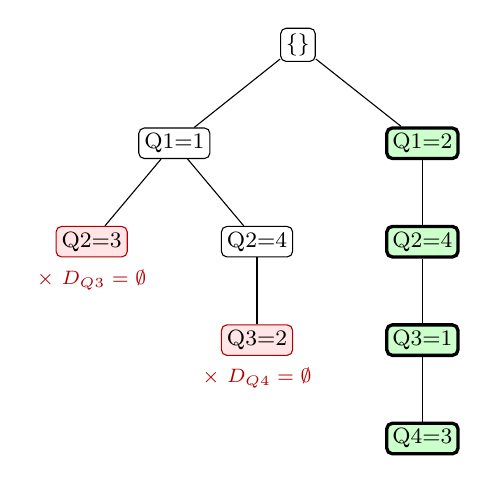
\begin{tikzpicture}[scale=1.0, every node/.style={transform shape}, bn/.style={draw, rounded corners=2pt, font=\footnotesize, inner sep=2pt}]
\node[bn] (b1) at (2.62,0.00) {$\{\}$};
\node[bn] (b2) at (1.05,-1.25) {Q1$=$1};
\node[bn, fill=red!10, draw=red!70!black] (b3) at (0.00,-2.50) {Q2$=$3};
\node[font=\scriptsize, text=red!70!black, below=1pt of b3] {$\times$ $D_{Q3}=\emptyset$};
\draw (b2) -- (b3);
\node[bn] (b4) at (2.10,-2.50) {Q2$=$4};
\node[bn, fill=red!10, draw=red!70!black] (b5) at (2.10,-3.75) {Q3$=$2};
\node[font=\scriptsize, text=red!70!black, below=1pt of b5] {$\times$ $D_{Q4}=\emptyset$};
\draw (b4) -- (b5);
\draw (b2) -- (b4);
\draw (b1) -- (b2);
\node[bn, fill=green!20, very thick] (b6) at (4.20,-1.25) {Q1$=$2};
\node[bn, fill=green!20, very thick] (b7) at (4.20,-2.50) {Q2$=$4};
\node[bn, fill=green!20, very thick] (b8) at (4.20,-3.75) {Q3$=$1};
\node[bn, fill=green!20, very thick] (b9) at (4.20,-5.00) {Q4$=$3};
\draw (b8) -- (b9);
\draw (b7) -- (b8);
\draw (b6) -- (b7);
\draw (b1) -- (b6);
\end{tikzpicture}
\end{adjustbox}
\end{center}Solution: $Q_1=2$, $Q_2=4$, $Q_3=1$, $Q_4=3$ (its mirror image $(3,1,4,2)$ is the other solution).
\end{solbox}
\question{10}The constraint graph below has only binary constraints and no variable is assigned initially. For each independent scenario, list every variable whose domain \emph{might} change.\begin{center}
\begin{adjustbox}{max width=\linewidth}
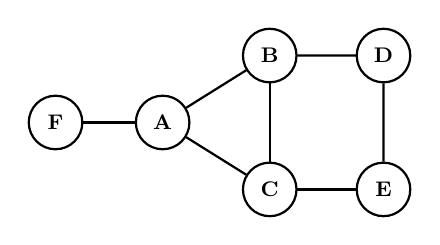
\begin{tikzpicture}[scale=0.85, every node/.style={transform shape}, cv/.style={draw, thick, circle, minimum size=8mm, inner sep=0pt, font=\small\bfseries}]
\node[cv] (A) at (0.00,1.20) {A};
\node[cv] (B) at (1.60,2.20) {B};
\node[cv] (C) at (1.60,0.20) {C};
\node[cv] (F) at (-1.60,1.20) {F};
\node[cv] (D) at (3.30,2.20) {D};
\node[cv] (E) at (3.30,0.20) {E};
\draw[thick] (A) to[] (B);
\draw[thick] (A) to[] (C);
\draw[thick] (A) to[] (F);
\draw[thick] (B) to[] (C);
\draw[thick] (B) to[] (D);
\draw[thick] (C) to[] (E);
\draw[thick] (D) to[] (E);
\end{tikzpicture}
\end{adjustbox}
\end{center}
\subq{(a)}A value is assigned to A and forward checking is run for A.
\begin{solbox}
Neighbours of A: \textbf{B, C, F}.
\end{solbox}
\subq{(b)}A is assigned and forward checking is run; then B is assigned and forward checking is run for B.
\begin{solbox}
Unassigned neighbours of B: \textbf{C, D}.
\end{solbox}
\subq{(c)}A is assigned and arc consistency is enforced.
\begin{solbox}
Propagation reaches the whole connected component: \textbf{B, C, D, E, F}.
\end{solbox}
\subq{(d)}A is assigned and arc consistency is enforced; then B is assigned and arc consistency is enforced again.
\begin{solbox}
\textbf{C, D, E}: propagation from B continues through unassigned variables only. F is reachable only through A, whose single value is already consistent, so A cannot change and no arc into F is re-examined.
\end{solbox}
\question{11}Answer the following questions briefly.
\subq{(a)}Describe the ``laws of thought'' approach with a syllogism, and give the two obstacles the lecture mentions.
\begin{solbox}
Irrefutable reasoning: \emph{All men are mortal; Socrates is a man; so Socrates is mortal}. Obstacles: not all intelligent behaviour is mediated by logic, and solving a problem ``in principle'' differs from solving it in practice (intractability).
\end{solbox}
\subq{(b)}On a 4-connected grid, compare the number of leaves of a depth-20 search tree with the number of distinct states within 20 steps (about $2d^2$). What does this say about tree-search vs graph-search?
\begin{solbox}
$4^{20}\approx10^{12}$ leaves vs $\approx800$ states: almost all nodes are redundant paths, so graph-search (remembering reached states) turns an intractable search into an easy one.
\end{solbox}
\subq{(c)}In simulated annealing a successor is $\Delta E=-3$ worse than the current state. Compute its acceptance probability at $T=10$, $3$, $1$. Why is simulated annealing better than plain hill climbing?
\begin{solbox}
$T=10$: $e^{-3/10}=0.741$, $T=3$: $e^{-3/3}=0.368$, $T=1$: $e^{-3/1}=0.050$. Early random downhill moves let it escape local maxima; as $T$ decreases it behaves like hill climbing.
\end{solbox}
\subq{(d)}With perfect move ordering, how many nodes does alpha-beta examine? Evaluate the effective branching factor for chess ($b\approx35$) and name two move-ordering techniques.
\begin{solbox}
$O(b^{m/2})$, effective branching factor $\sqrt{35}\approx5.9$. Killer-move heuristic; transposition tables.
\end{solbox}
\question{12}True or false?
For each statement, circle \textbf{T} or \textbf{F} and justify your answer in one or two sentences (an answer without a correct justification earns no credit).
\subq{1.}In graph search the frontier separates the expanded (interior) region from the unreached (exterior) region. \hfill \textbf{T \quad F}
\begin{solbox}
\T. Graph-search separation property: every path to an unreached state passes through the frontier.
\end{solbox}
\subq{2.}For BFS, memory is a bigger problem than execution time. \hfill \textbf{T \quad F}
\begin{solbox}
\T. All generated nodes are kept: $O(b^d)$ memory runs out first.
\end{solbox}
\subq{3.}A* graph search with a consistent heuristic never needs to re-expand a state. \hfill \textbf{T \quad F}
\begin{solbox}
\T. The first time a state is expanded it is on an optimal path, so no cheaper path is found later.
\end{solbox}
\subq{4.}A* with an inadmissible heuristic can never return an optimal solution. \hfill \textbf{T \quad F}
\begin{solbox}
\F. It may, e.g.\ if all nodes on an optimal path have admissible $h$ values.
\end{solbox}
\subq{5.}For the 8-puzzle, $h=\max\{2,h_{\text{Manhattan}}\}$ is admissible. \hfill \textbf{T \quad F}
\begin{solbox}
\F. At the goal $h=2>0$.
\end{solbox}
\subq{6.}For the 8-puzzle, $h=\min\{2,h_{\text{Manhattan}}\}$ is admissible. \hfill \textbf{T \quad F}
\begin{solbox}
\T. $h\le h_{\text{Manhattan}}\le h^*$.
\end{solbox}
\subq{7.}Pruning in expectimax is possible only if the leaf values are known to lie in a bounded range. \hfill \textbf{T \quad F}
\begin{solbox}
\T. Otherwise an unseen outcome could always raise the average above any bound.
\end{solbox}
\subq{8.}In UCB1, increasing $C$ makes MCTS more exploratory. \hfill \textbf{T \quad F}
\begin{solbox}
\T. $C$ scales the exploration term $\sqrt{\ln N/n_i}$.
\end{solbox}
\subq{9.}The least-constraining-value heuristic tries first the value that rules out the most choices for the neighbours. \hfill \textbf{T \quad F}
\begin{solbox}
\F. It prefers the value ruling out the \emph{fewest} (fail-last).
\end{solbox}
\subq{10.}Any constraint over more than two variables can be transformed into binary constraints. \hfill \textbf{T \quad F}
\begin{solbox}
\T. As stated in the lecture (e.g.\ by introducing auxiliary variables).
\end{solbox}
\end{document}